\documentclass[11pt,letterpaper,final]{report}
\usepackage[utf8]{inputenc}
\usepackage[francais]{babel}
\usepackage[T1]{fontenc}
\usepackage{amsmath}
\usepackage{amsfonts}
\usepackage{amssymb}
\usepackage{graphicx}
\usepackage{lmodern}
\usepackage[left=2.54cm,right=2.54cm,top=2.54cm,bottom=2.54cm]{geometry}
\begin{document}
\chapter{Cross validation entre les différentes plateformes de simulations}
Dans ce chapitre, les simulateurs seront comparés selon les paramètres des simulations critiques (courant dans les électroaimants, tension aux bornes des électroaimants, courant d'entrée, tension du bus CC, etc.). Les différences seront analysées selon les sous-modèles implantés, qui seront détaillés plus loin dans cet ouvrage. Les sous-modèles se séparent en plusieurs catégories, soit les simulations représentant l'AFE, celles représentant le convertisseur CC-CC et celles représentant un montage avec un AFE et un convertisseur CC-CC. Il est à noté que les temps de simulation qui seront employés pour fins d'analyse sont de 50$\mu$s, de 5$\mu$s et de 1$\mu s$. 

\section{Différences entre PSIM et SPS}
Cette section va décrire quelques différences découvertes au sein de deux systèmes de simulations utilisés pour simuler les différents modèles implantés lors de ce projet, soit PSIM et SPS. En premier lieu, PSIM est un système de simulation qui simule en continu tandis que pour nos simulations sur SPS tout est discrétisé. De plus,les algorithmes utilisés pour résoudre les simulations ne sont pas les mêmes. Lors d'un passage par zéro, SPS ne réagit pas de la même manière que PSIM ce qui peut faire apparaître des différences dans les résultats. Il faut comprendre que les différences encourues diminues à fur à mesure que le pas de calcul utilisé diminue.  

Par rapport aux éléments utilisés, plusieurs différences ont été aperçu. Commençons par les IGBT, qui sont modélisé comme parfait sur SPS et non sur PSIM. De sorte, que sur PSIM il y a de faibles pertes par commutation ce que SPS n'a pas. De plus, les modèles implantés sur SPS ont un snubber RC tandis que sur PSIM il y en a pas. Pour contrer cette différence, une charge RC a été rajouté en parallèle à chaque IGBT avec les mêmes paramètres soit 50k$\Omega$.

Les relay utilisés diffère entre les deux simulations. Sur SPS, il suffit juste d'indiquer les seuils voulus ce qui fait en sorte que le relay réagit instantanément ou presque lorsque le seuil est atteint(En fonction du pas de calcul). Sur PSIM en plus d'indiquer le seuil, il faut indiquer d'autres paramètres, entre autres, 'Operate time' et 'Release time' qui indique le temps d'attente entre la détection de l'atteinte du seuil et le changement d'état. Ces valeurs doivent correspondre à deux fois le pas de calcul ou plus.



\section{Pont DCP/DCN: Validation PSIM/SPS}
\subsection{Hacheur 4 quadrants}
Le hacheur 4 quadrants, à proprement parlé, est constitué de 4 interrupteurs IGBT commandés au moyen d'une régulation MLI. La figure~\ref{hach} présente une représentation schématique d'un tel convertisseur. Ce type de montage est un montage de base utilisé afin de valider le concept de fonctionnement d'un convertisseur CC-CC et afin d'établir la méthodologie de comparaison des simulations.

\begin{figure}[htb]
\centering
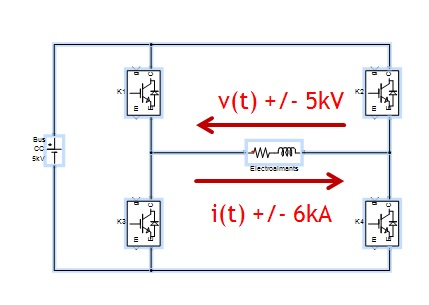
\includegraphics[scale=1]{Fig/Hacheur4Quadrants/Hacheur.jpg}
\caption{Pont en H a 4 intérrupteurs}.
\label{hach}
\end{figure}

\subsubsection{Vérification pour un pas de calcul de 50$\mu$s}
Cette section présente les courbes d'intérêt pour un pas de calcul discret de 50$\mu$s. La figure \ref{comp_PSIM_SPS} présente le courant à la charge sur PSIM et SPS pour un pas de calcul de 50 $\mu$s. Sur cette figure, on remarque que les différences entre les deux courants avoisinent les 25A. Aussi, la courbe de PSIM est décalée d'environ 150$\mu$s vers la droite par rapport à celle de SPS. On remarque que les résultats des simulations sont décalés jusqu'à 100A de la valeur de référence voulu. 

\begin{figure}[htb]
\centering
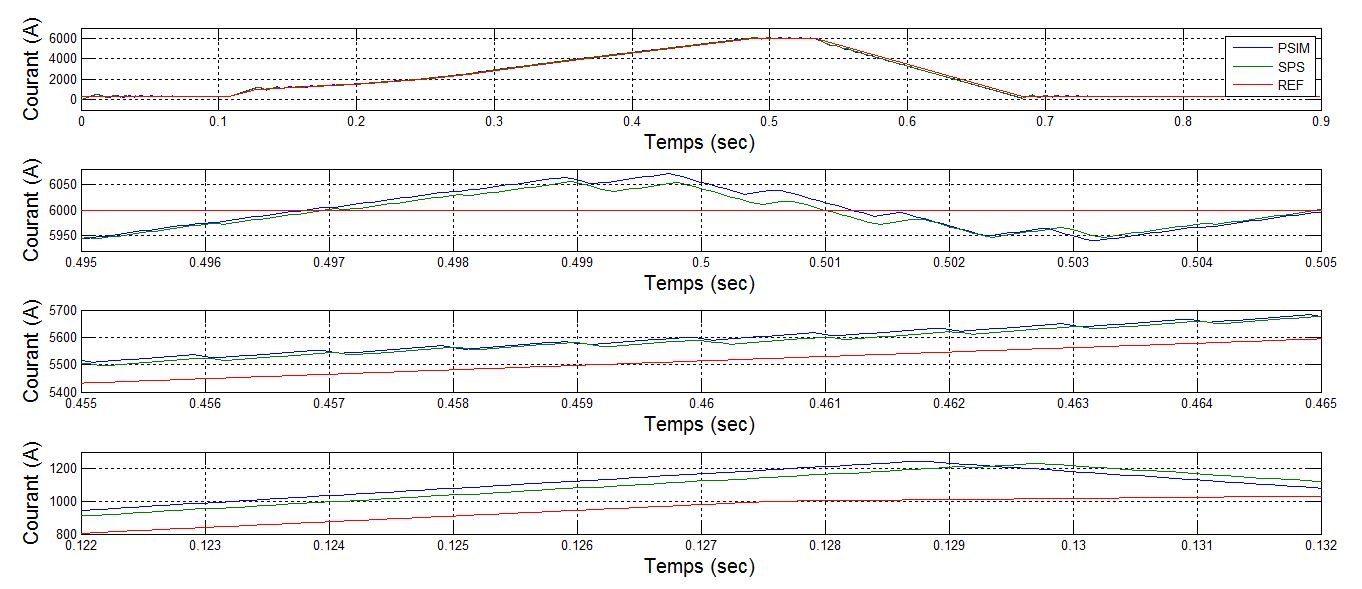
\includegraphics[scale=0.5]{Fig/Hacheur4Quadrants/HacheurCourantCharge50u.jpg}
\caption{Courant à la charge sur PSIM et SPS pour un pas de calcul de 50$\mu$s}.
\label{comp_PSIM_SPS}
\end{figure}
Sur la figure~\ref{err_cou} qui présente la tension à la charge, nous observons que les deux simulations donne les mêmes résultats à part le fait que le résultat de SPS est décalé d'environs 100$\mu$s vers la droite de celle de PSIM.

\begin{figure}[htb]
\centering
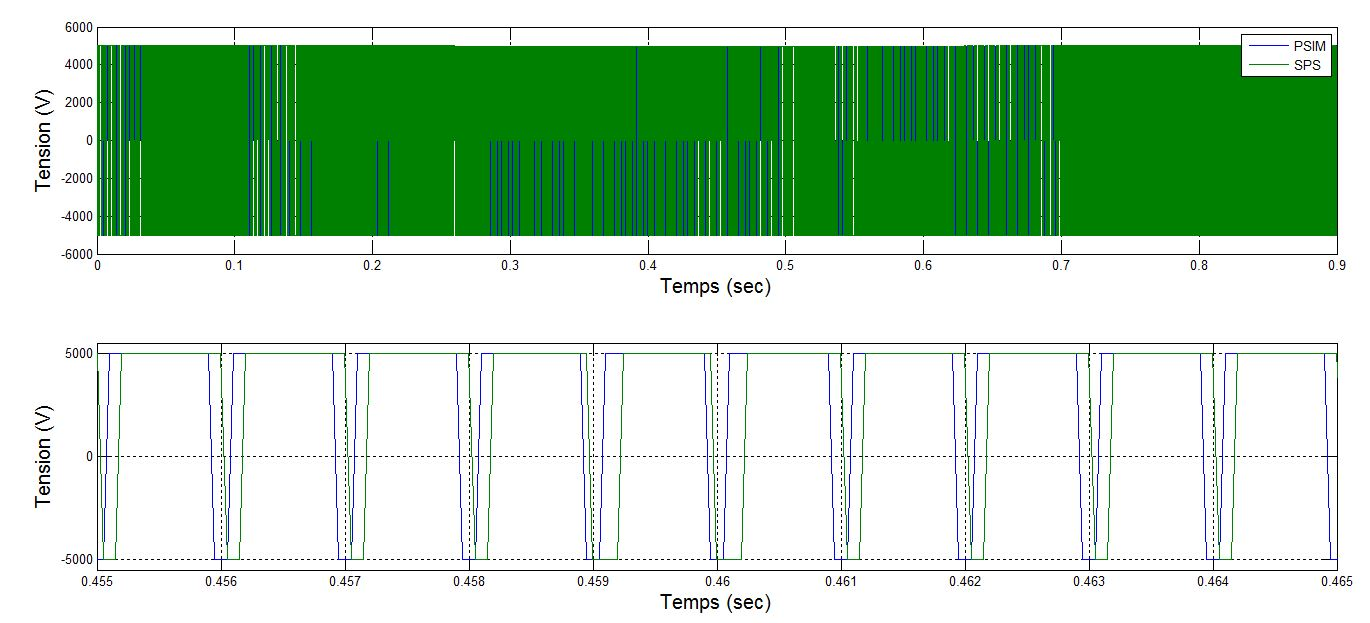
\includegraphics[scale=0.5]{Fig/Hacheur4Quadrants/HacheurTensionCharge50u.jpg}
\caption{Tension aux bornes de la charge sur PSIM et SPS pour un pas de calcul de 50$\mu$s}
\label{err_cou}
\end{figure}

La figure~\ref{hc_IG_ten_50} représente la tension aux bornes d'un IGBT pour le hacheur 4 quadrants. On remarque que les résultats sont pas toutes identiques mais la fréquence est la même. La différence observé est dû à l'algorithme de résolution de chacune des simulations. Sur SPS la simulation est discrétisé et a un passage par zéro l'algorithme change d'euler a une méthode trapézoïdale. Tandis que sur PSIM la simulation est résolu en continu.
\begin{figure}[htb]
\centering
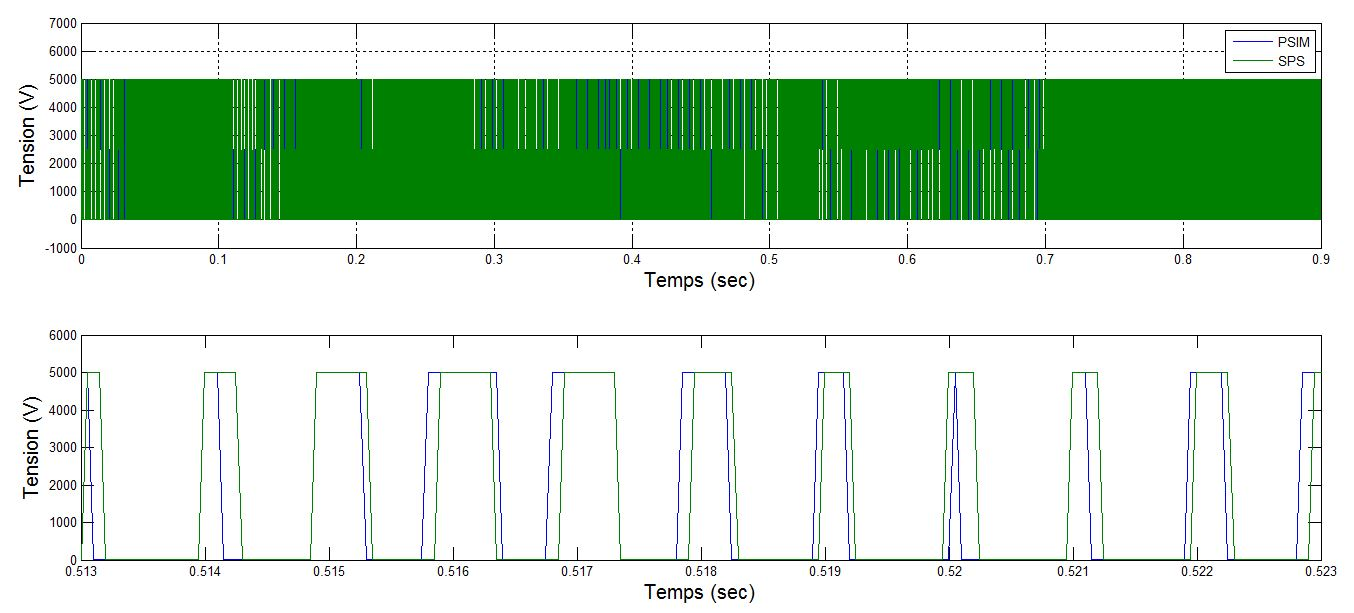
\includegraphics[scale=0.5]{Fig/Hacheur4Quadrants/HacheurTensionIGBT50u.jpg}
\caption{Tension aux bornes d'un IGBT sur PSIM et SPS pour un pas de calcul de 50$\mu$s}
\label{hc_IG_ten_50}
\end{figure}

\clearpage
\subsubsection{Vérification pour un pas de calcul de 5$\mu$s}
Cette section présente les courbes d'intérêt pour un pas de calcul discret de 5$\mu$s. À ce pas de calcul le résultat est beaucoup plus précis. La figure~\ref{hc_cou_ch_5}
montre le courant à charge pour un pas de 5$\mu$s.  Le courant à la charge observé en différentes période entre PSIM et SPS est en phase. On remarque par contre que l'oscillation de courant de SPS est décalé d'environs 10A, mais qu'elles suivent très bien la référence de courant voulu avec une différence d'environs 18A.
\begin{figure}[htb]
\centering
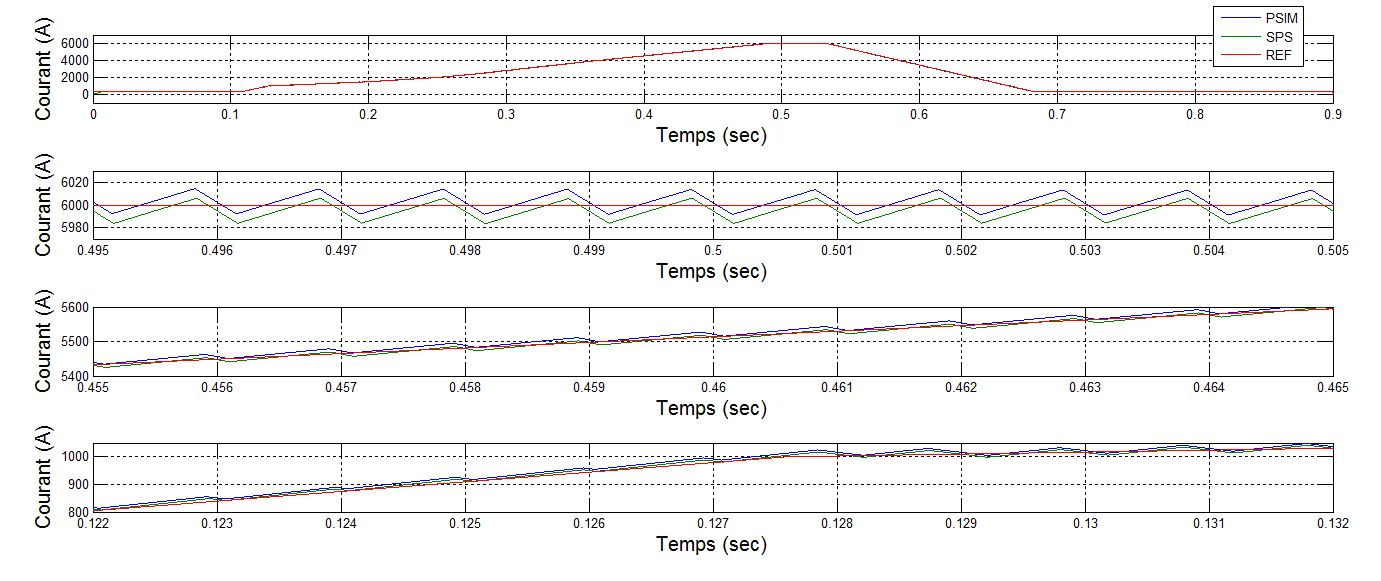
\includegraphics[scale=0.5]{Fig/Hacheur4Quadrants/HacheurCourantCharge5u.jpg}
\caption{Courant traversant la charge sur PSIM et SPS pour un pas de calcul de 5$\mu$s}
\label{hc_cou_ch_5}
\end{figure}
Les deux figures suivantes~\ref{hc_ten_ch_5} et ~\ref{hc_IG_ten_5} qui représente la tension à la charge et aux bornes de l'IGBT ont des courbes entre PSIM et SPS qui se superpose très bien, qui donne pratiquement le même résultat.


\begin{figure}[htb]
\centering
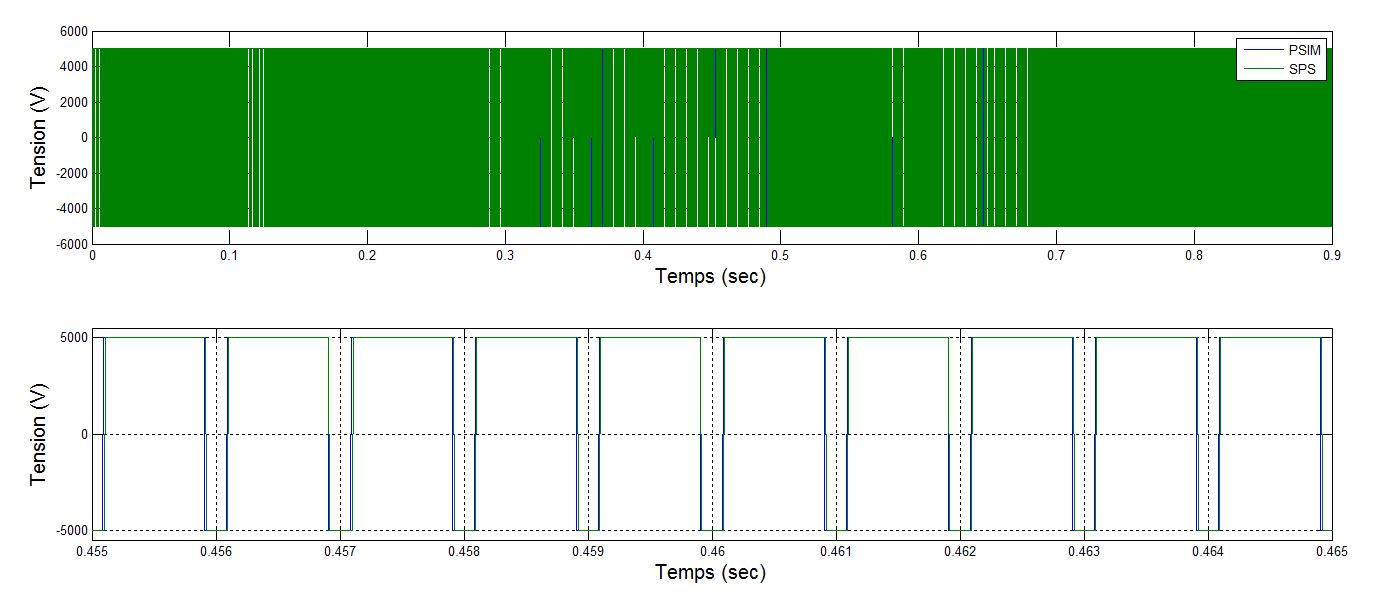
\includegraphics[scale=0.5]{Fig/Hacheur4Quadrants/HacheurTensionCharge5u.jpg}
\caption{Tension aux bornes de la charge sur PSIM et SPS pour un pas de calcul de 5$\mu$s}
\label{hc_ten_ch_5}
\end{figure}


\begin{figure}[htb]
\centering
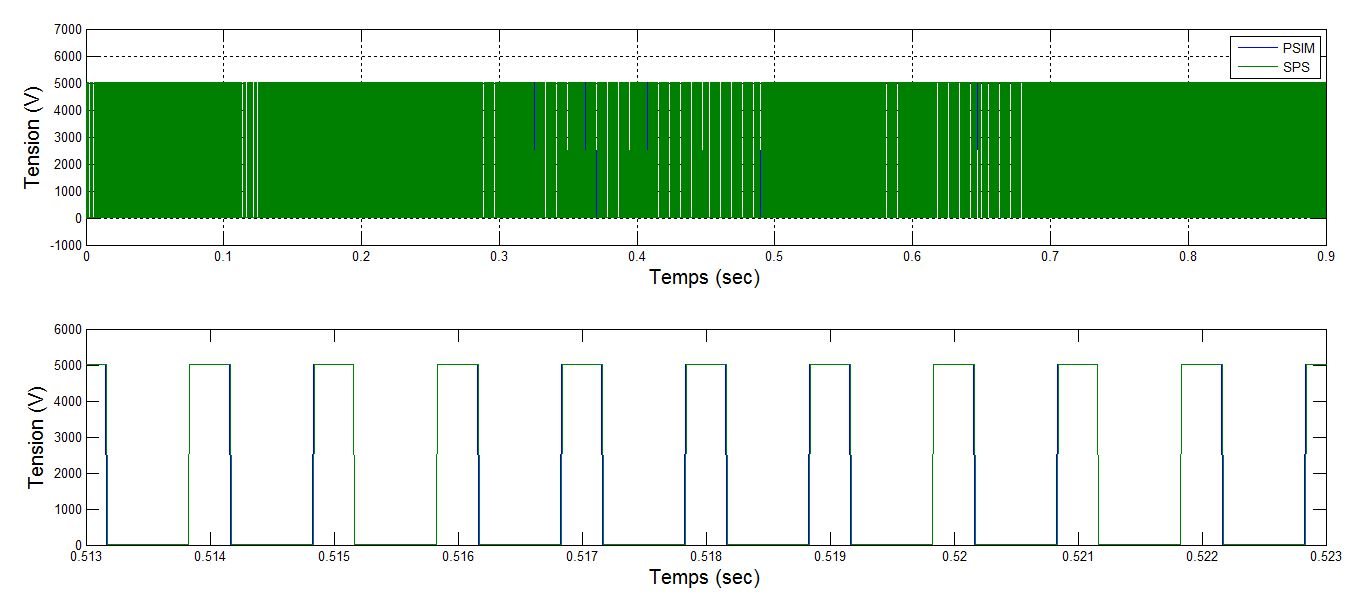
\includegraphics[scale=0.5]{Fig/Hacheur4Quadrants/HacheurTensionIGBT5u.jpg}
\caption{Tension aux bornes d'un IGBT sur PSIM et SPS pour un pas de calcul de 5$\mu$s}
\label{hc_IG_ten_5}
\end{figure}

\clearpage
\subsubsection{Vérification pour un pas de calcul de 1$\mu$s}
Cette section présente les courbes d'intérêt pour un pas de calcul discret de 1$\mu$s. On remarque que les résultats des figures~\ref{hc_cou_ch_1}, ~\ref{hc_ten_ch_1}, ~\ref{hc_IG_cou_1} et ~\ref{hc_IG_ten_1} qui représentent le courant à la charge, la tension à la charge, le courant et tension au niveau de IGBT à un pas de calcul de 1$\mu$s, donne les mêmes résultats qui ceux obtenu pour un pas de 5$\mu$s mais avec une meilleur précision. 


\begin{figure}[htb]
\centering
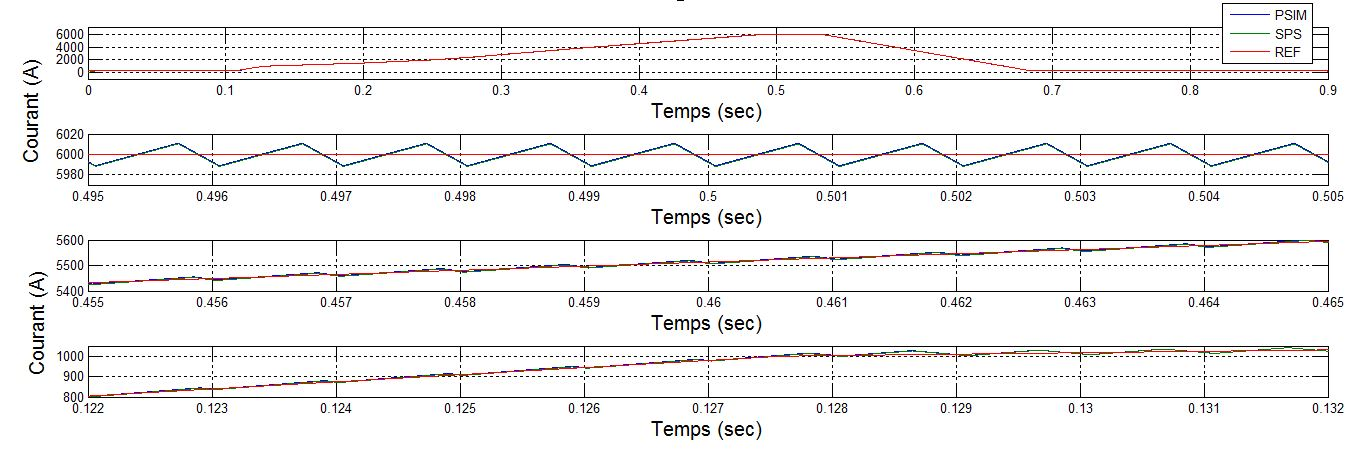
\includegraphics[scale=0.5]{Fig/Hacheur4Quadrants/HacheurCourantCharge1u.jpg}
\caption{Courant traversant la charge sur PSIM et SPS pour un pas de calcul de 1$\mu$s}
\label{hc_cou_ch_1}
\end{figure}


\begin{figure}[htb]
\centering
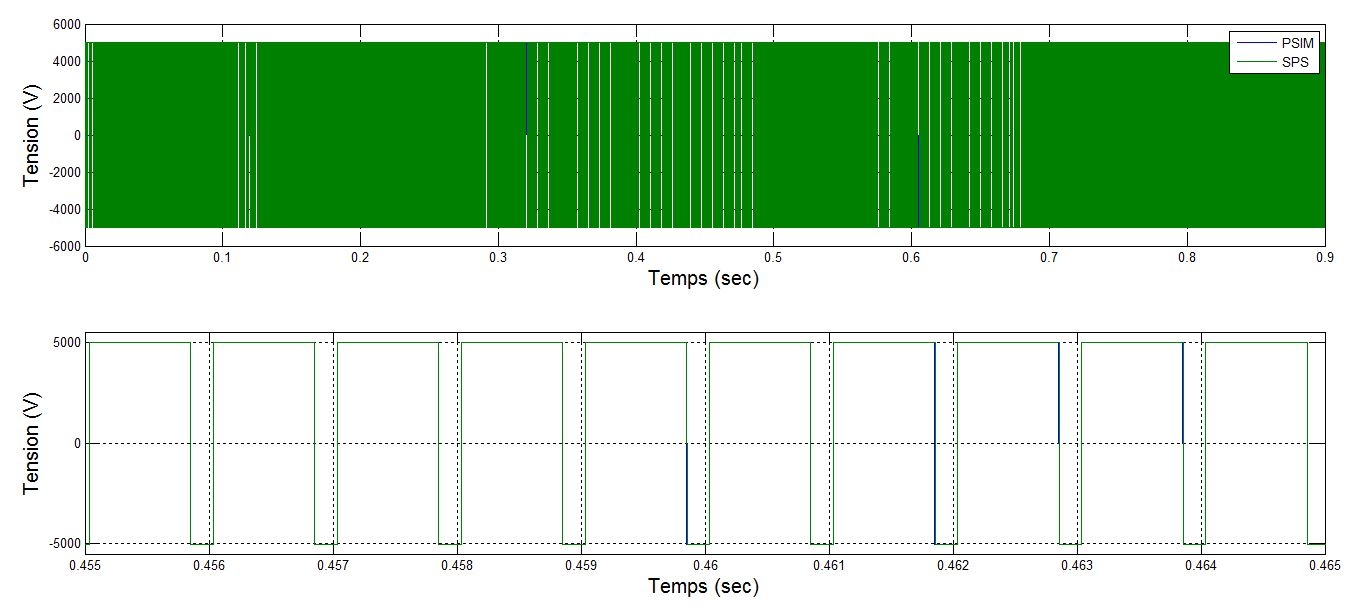
\includegraphics[scale=0.5]{Fig/Hacheur4Quadrants/HacheurTensionCharge1u.jpg}
\caption{Tension aux bornes de la charge sur PSIM et SPS pour un pas de calcul de 1$\mu$s}
\label{hc_ten_ch_1}
\end{figure}


\begin{figure}[htb]
\centering
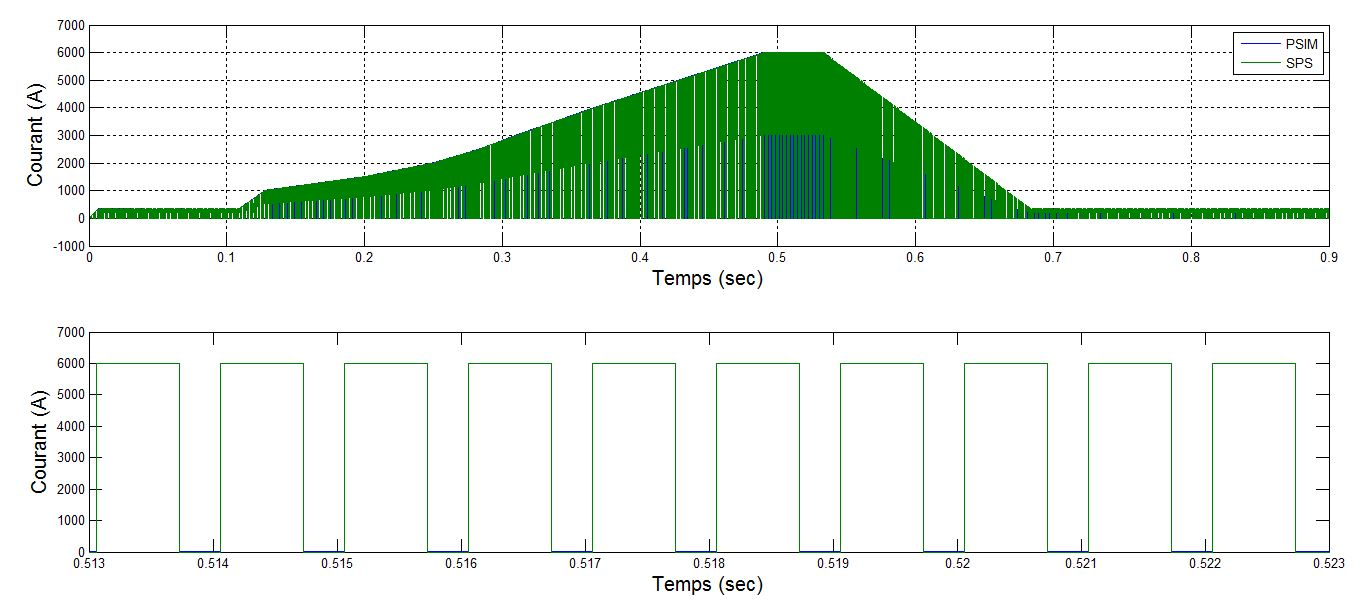
\includegraphics[scale=0.5]{Fig/Hacheur4Quadrants/HacheurCourantIGBT1u.jpg}
\caption{Courant traversant un IGBT sur PSIM et SPS pour un pas de calcul de 1$\mu$s}
\label{hc_IG_cou_1}
\end{figure}

\begin{figure}[htb]
\centering
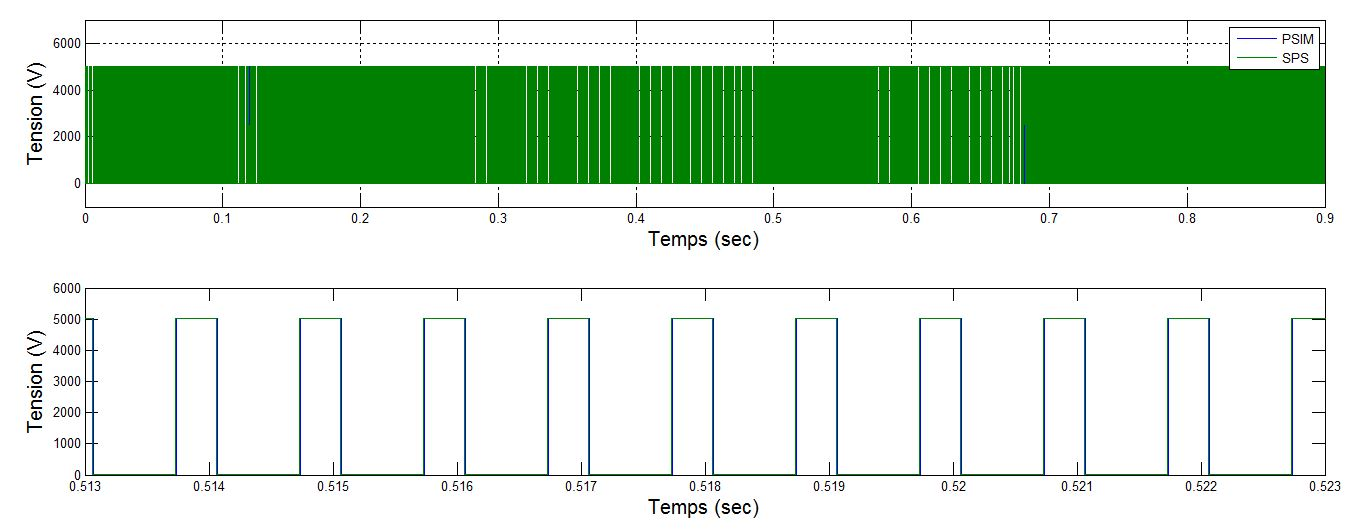
\includegraphics[scale=0.5]{Fig/Hacheur4Quadrants/HacheurTensionIGBT1u.jpg}
\caption{Tension aux bornes d'un IGBT sur PSIM et SPS pour un pas de calcul de 1$\mu$s}
\label{hc_IG_ten_1}
\end{figure}


\clearpage

\subsection{DCP/DCN}
Le DCP/DCN est un convertisseur CC-CC, qui représente un système plus complexe du fonctionnement du hacheur 4 quadrants. Il est composé de 24 interrupteurs IGBT/DIODE commandé avec une commande MLI ainsi que de 12 diodes de retour. La figure~\ref{DC_DP} représente une configuration schématique simple d'un tel système.

\begin{figure}[htb]
\centering
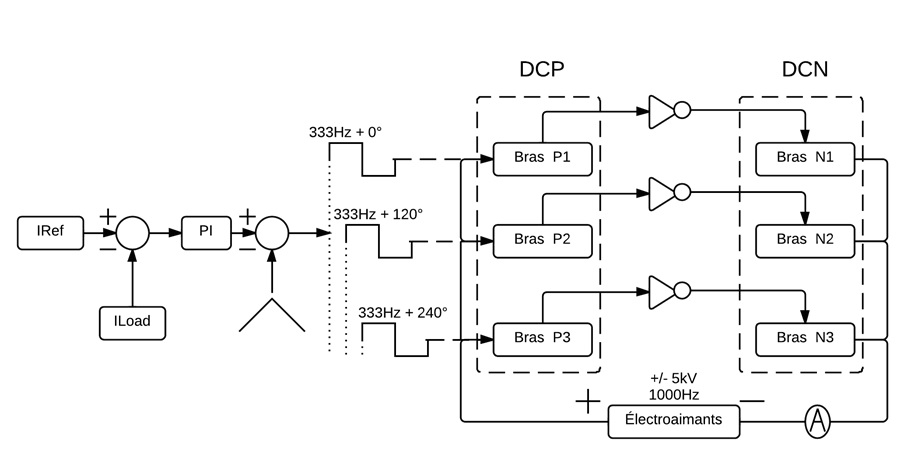
\includegraphics[scale=0.5]{Fig/DCPDCN/DCP.jpg}
\caption{Schéma bloc du DCP/DCN avec une commande MLI à la charge}
\label{DC_DP}
\end{figure}

\subsubsection{Vérification à un pas de calcul de 50$\mu$s}
Cette section présente les courbes d'intérêt pour un pas de calcul discret de 50$\mu$s. La figure~\ref{DC_ch_cou_50} qui représente la courant à la charge à un pas de calcul de 50$\mu$s montre que le résultat de PSIM et SPS ne vont pas à la même fréquence, la fréquence de SPS est plus élevé que celle de PSIM. Par contre, ils sont décalés deulement d'environs 18A par rapport au courant de référence.



\begin{figure}[htb]
\centering
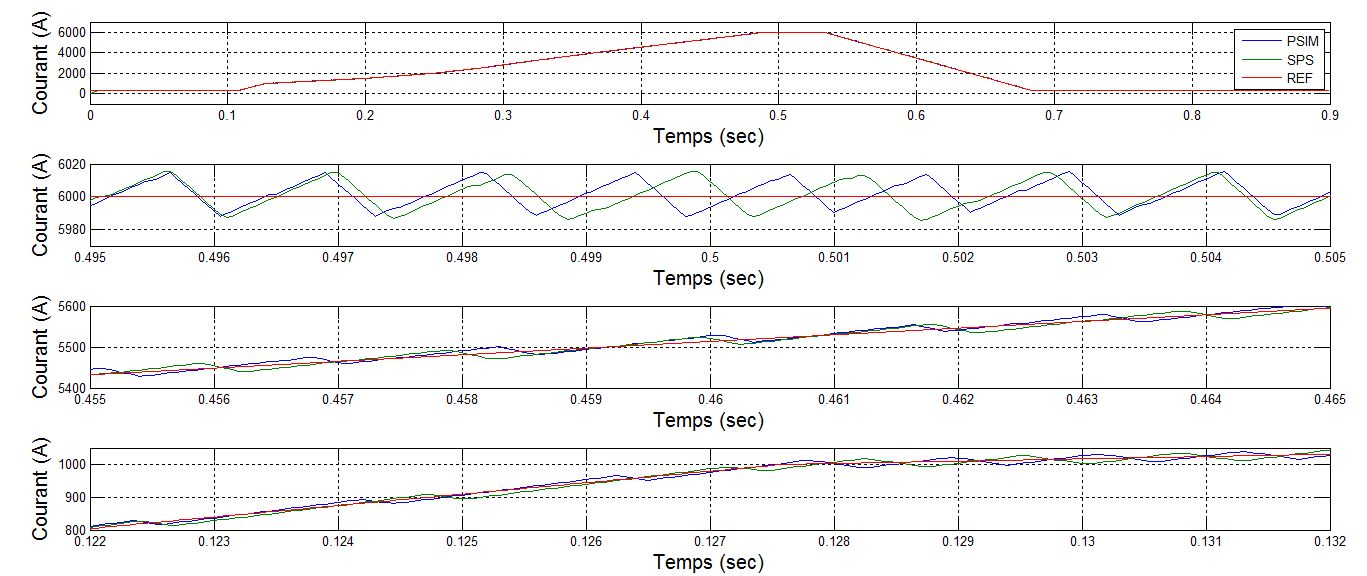
\includegraphics[scale=0.5]{Fig/DCPDCN/DCPCourantCharge50u.jpg}
\caption{Courant traversant la charge sur PSIM et SPS pour un pas de calcul de 50$\mu$s}
\label{DC_ch_cou_50}
\end{figure}

Les figures~\ref{DC_ch_ten_50},~\ref{DC_IG_cou_50} et ~\ref{DC_IG_ten_50} qui représentent la tension à la charge, et le courant et la tension au niveau d'un IGBT montre que les résultats comportent de nombreuses commutations non désirés et des dépassements.

\begin{figure}[htb]
\centering
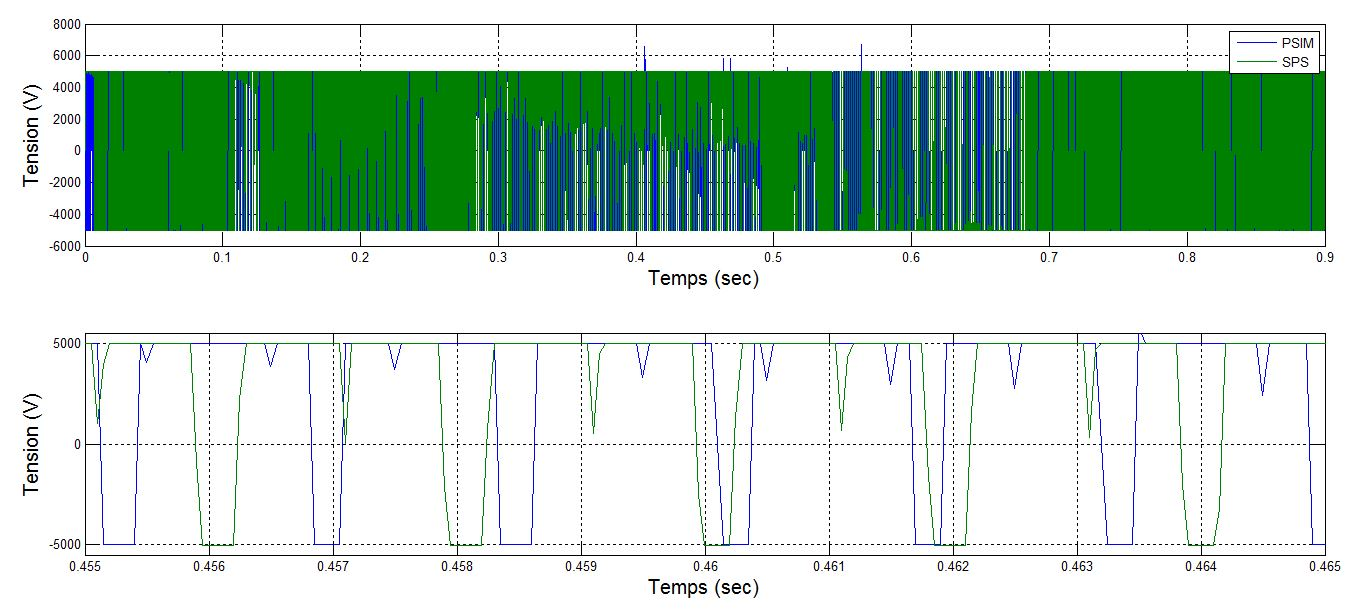
\includegraphics[scale=0.5]{Fig/DCPDCN/DCPTensionCharge50u.jpg}
\caption{Tension aux bornes de la charge sur PSIM et SPS pour un pas de calcul de 50$\mu$s}.
\label{DC_ch_ten_50}
\end{figure}

\begin{figure}[htb]
\centering
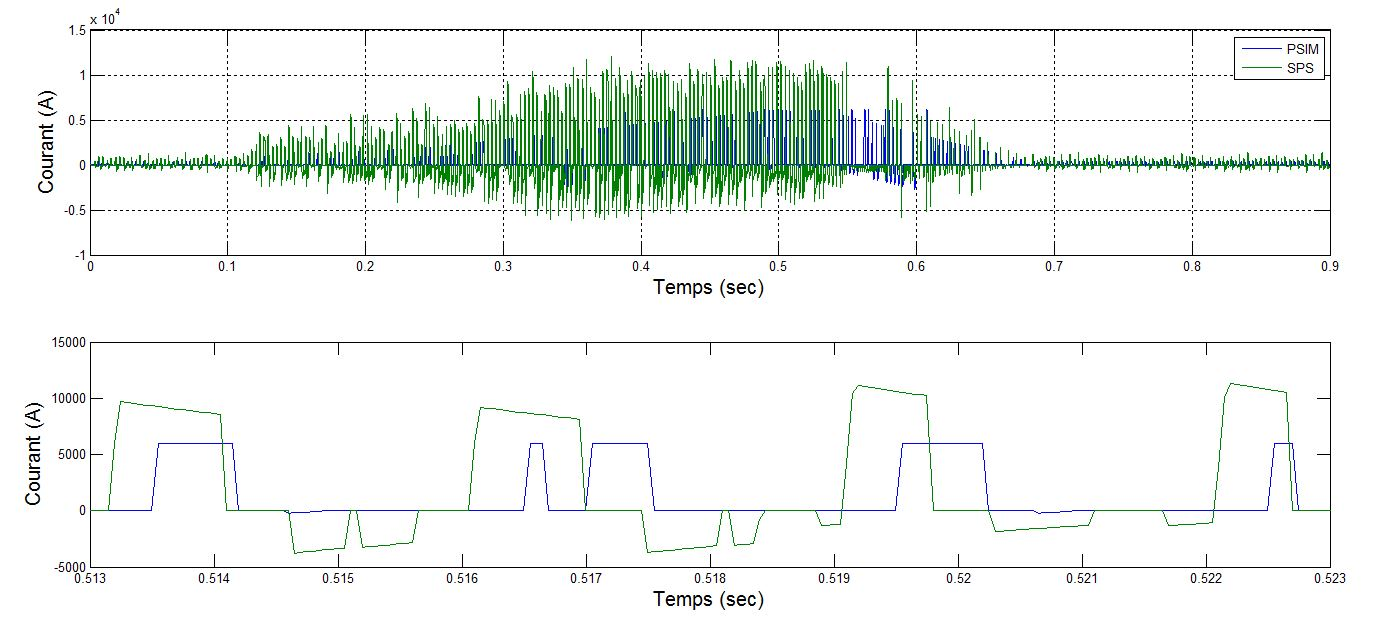
\includegraphics[scale=0.5]{Fig/DCPDCN/DCPCourantIGBT50u.jpg}
\caption{Courant traversant un IGBT sur PSIM et SPS pour un pas de calcul de 50$\mu$s}
\label{DC_IG_cou_50}
\end{figure}

\begin{figure}[htb]
\centering
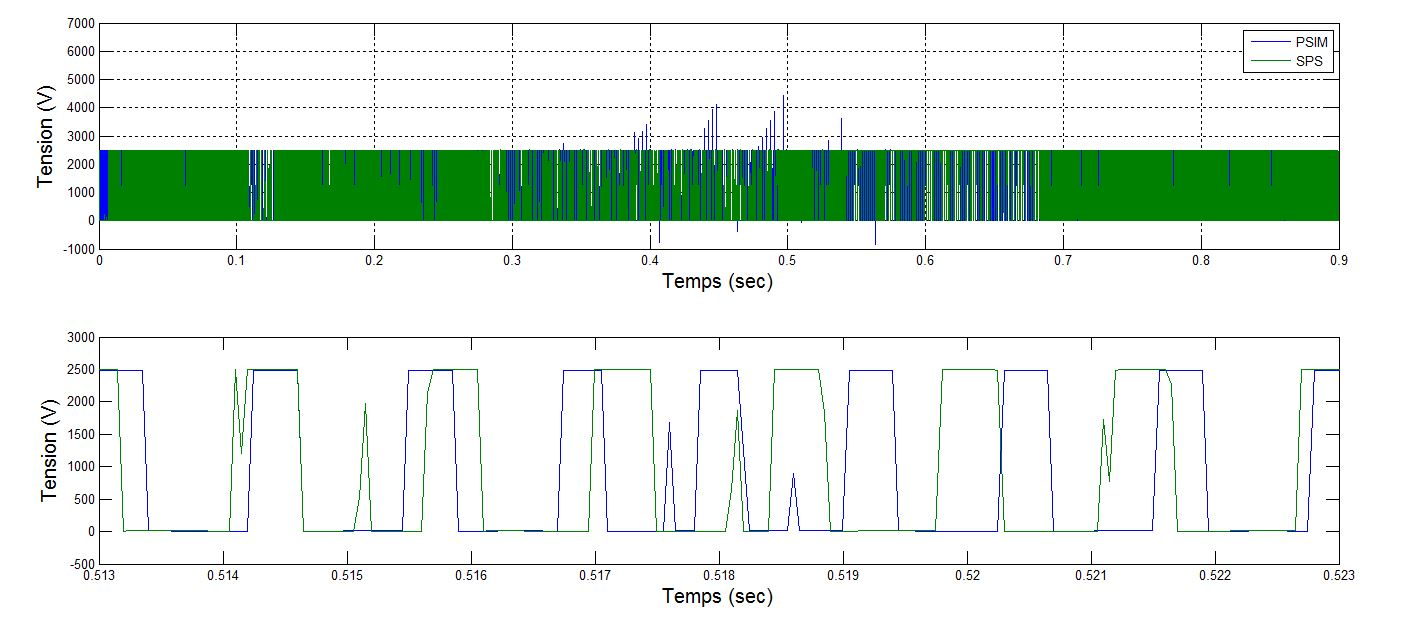
\includegraphics[scale=0.5]{Fig/DCPDCN/DCPTensionIGBT50u.jpg}
\caption{Tension au niveau d'un IGBT sur PSIM et SPS pour un pas de calcul de 50$\mu$s}
\label{DC_IG_ten_50}
\end{figure}


\clearpage

\subsubsection{Vérification à pas de calcul de 5$\mu$s}
Cette section présente les courbes d'intérêt pour un pas de calcul discret de 5$\mu$s. La figure~\ref{DC_ch_cou_5} qui représente le courant à la charge, montre un décalage de fréquence entre PSIM et SPS. 





\begin{figure}[htb]
\centering
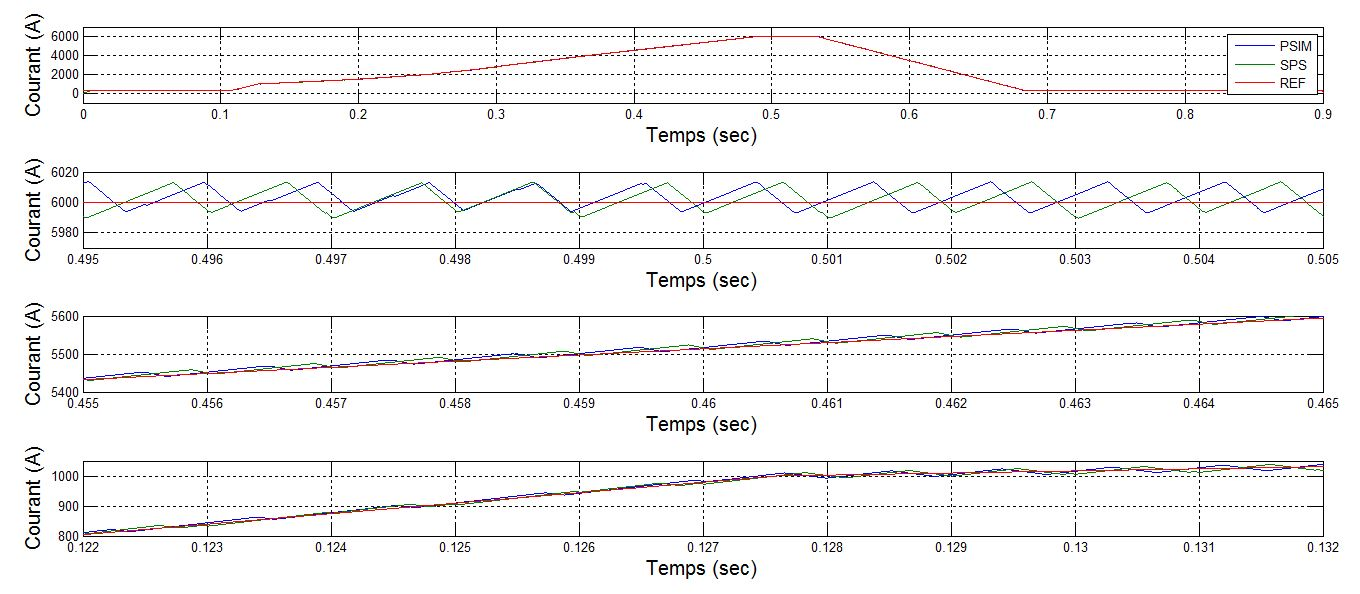
\includegraphics[scale=0.5]{Fig/DCPDCN/DCPCourantCharge5u.jpg}
\caption{Courant traversant la charge sur PSIM et SPS pour un pas de calcul de 5$\mu$s}
\label{DC_ch_cou_5}
\end{figure}
Sur les figures~\ref{DC_ch_ten_5} et ~\ref{DC_IG_ten_5} qui représente la tension sur la charge et l'IGBT, nous remarquons qu'il n'y a pas de dépassements sur la tension  mais qu'il y a des commutations non désirées. 

\begin{figure}[htb]
\centering
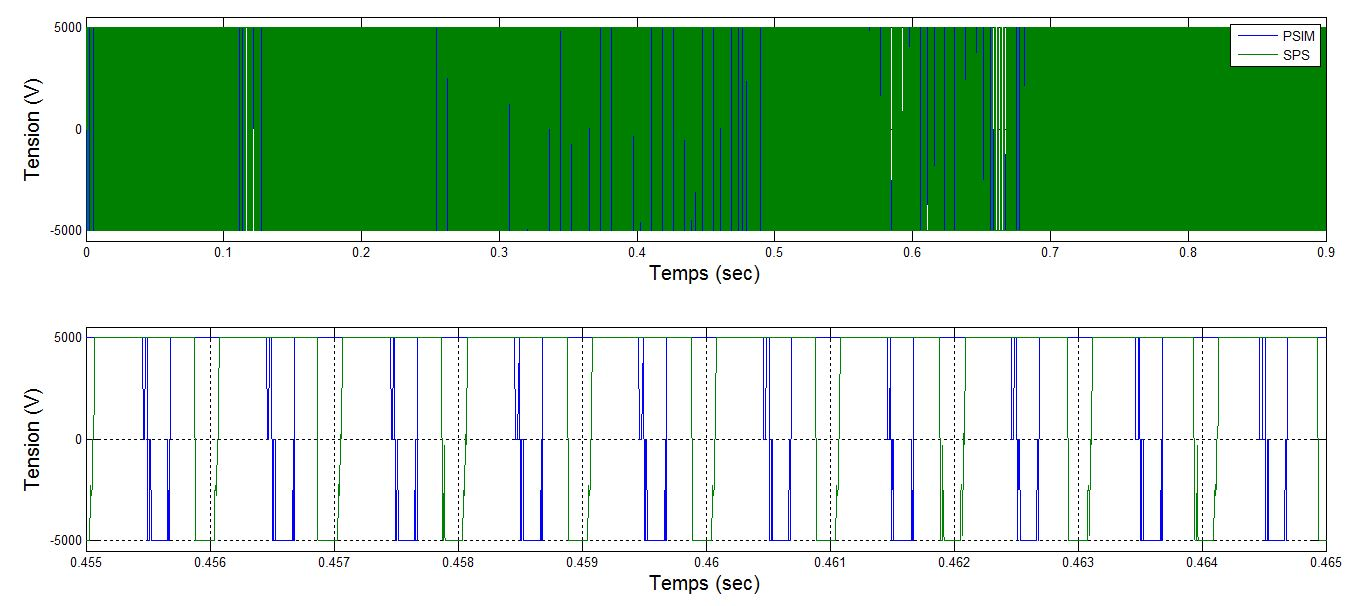
\includegraphics[scale=0.5]{Fig/DCPDCN/DCPTensionCharge5u.jpg}
\caption{Tension aux bornes de la charge sur PSIM et SPS pour un pas de calcul de 5$\mu$s}
\label{DC_ch_ten_5}
\end{figure}

La figure~\ref{DC_IG_cou_5} qui représente le courant au niveau de l'IGBT, nous remarquons que le résultat de SPS contient des dépassements qui ne sont pas présent sur le résultat de PSIM. Ce dépassement est causé par une différence au niveau des algorithmes utilisé.

\begin{figure}[htb]
\centering
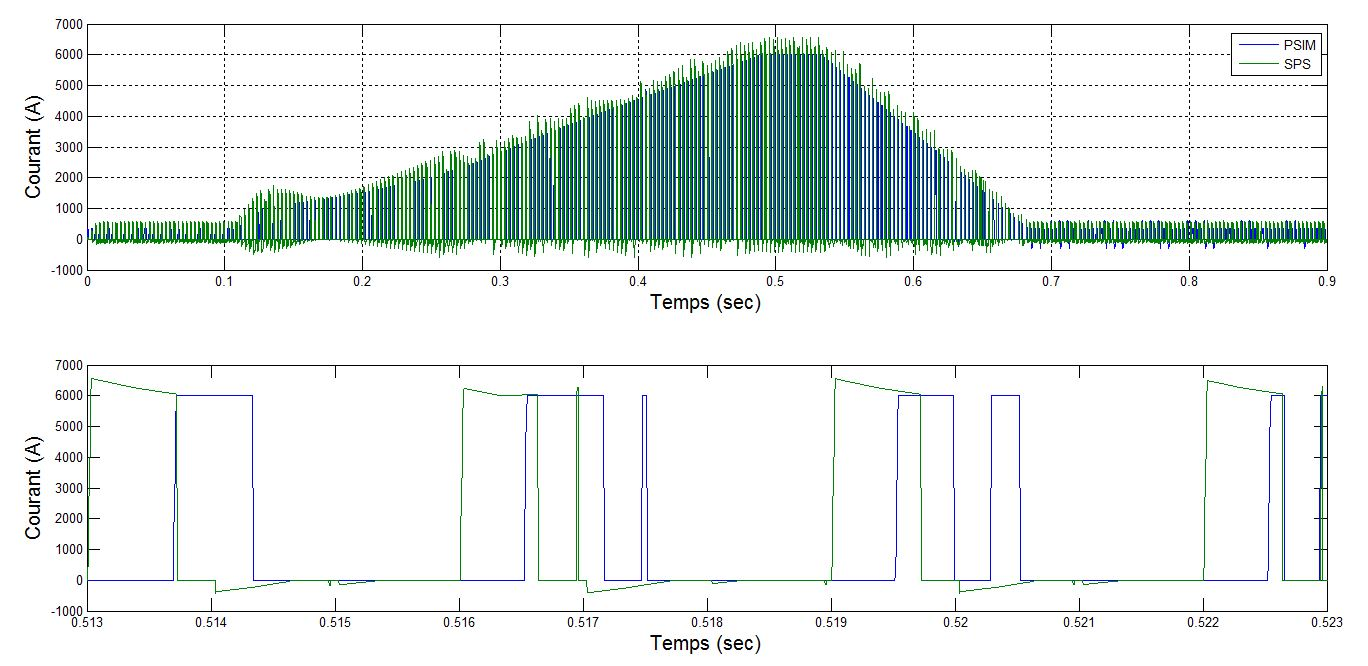
\includegraphics[scale=0.5]{Fig/DCPDCN/DCPCourantIGBT5u.jpg}
\caption{Courant traversant un IGBT sur PSIM et SPS pour un pas de calcul de 5$\mu$s}
\label{DC_IG_cou_5}
\end{figure}



\begin{figure}[htb]
\centering
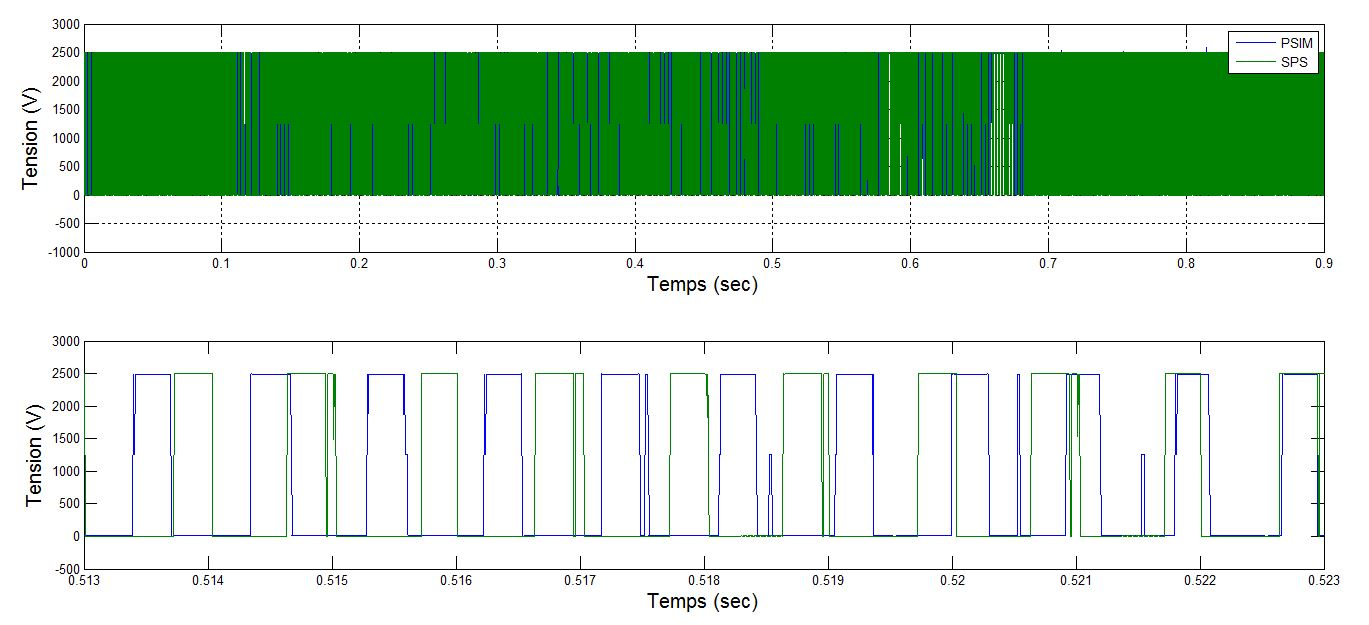
\includegraphics[scale=0.5]{Fig/DCPDCN/DCPTensionIGBT5u.jpg}
\caption{Tension traversant un IGBT sur PSIM et SPS pour un pas de calcul de 5$\mu$s}
\label{DC_IG_ten_5}
\end{figure}



\clearpage
\subsubsection{Vérification à un pas de calcul de 1us}
Cette section présente les courbes d'intérêt pour un pas de calcul discret de 1$\mu$s. La figure~\ref{DC_ch_cou_1} représente le courant à la charge pour un pas de calcul de 1$\mu$s. On remarque que le courant ne va pas à la même fréquence mais qu'il est décalé d'environs 18A par rapport au courant de référence.



\begin{figure}[htb]
\centering
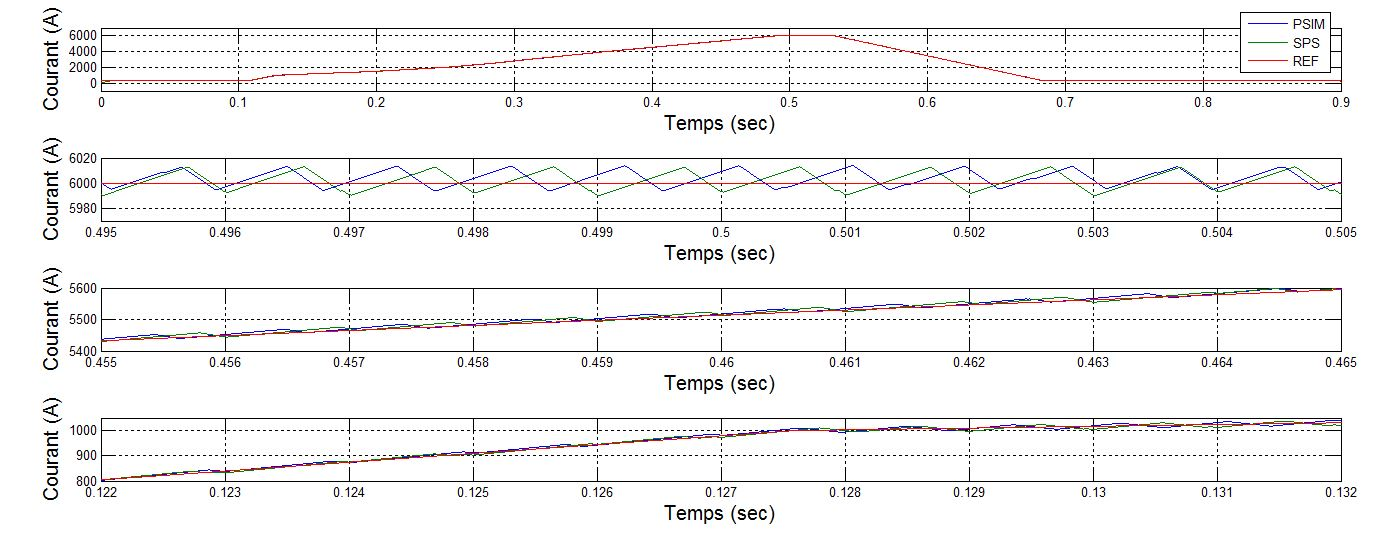
\includegraphics[scale=0.5]{Fig/DCPDCN/DCPCourantCharge1u.jpg}
\caption{Courant traversant la charge sur PSIM et SPS pour un pas de calcul de 1$\mu$s}
\label{DC_ch_cou_1}
\end{figure}

Les figures~\ref{DC_ch_ten_1}, ~\ref{DC_IG_cou_1} et ~\ref{DC_IG_ten_1} qui représentent la tension à la charge et la tension et le courant aux bornes de l'IGBT comportent des commutations non désiré mais ne contient pas de dépassements.

\begin{figure}[htb]
\centering
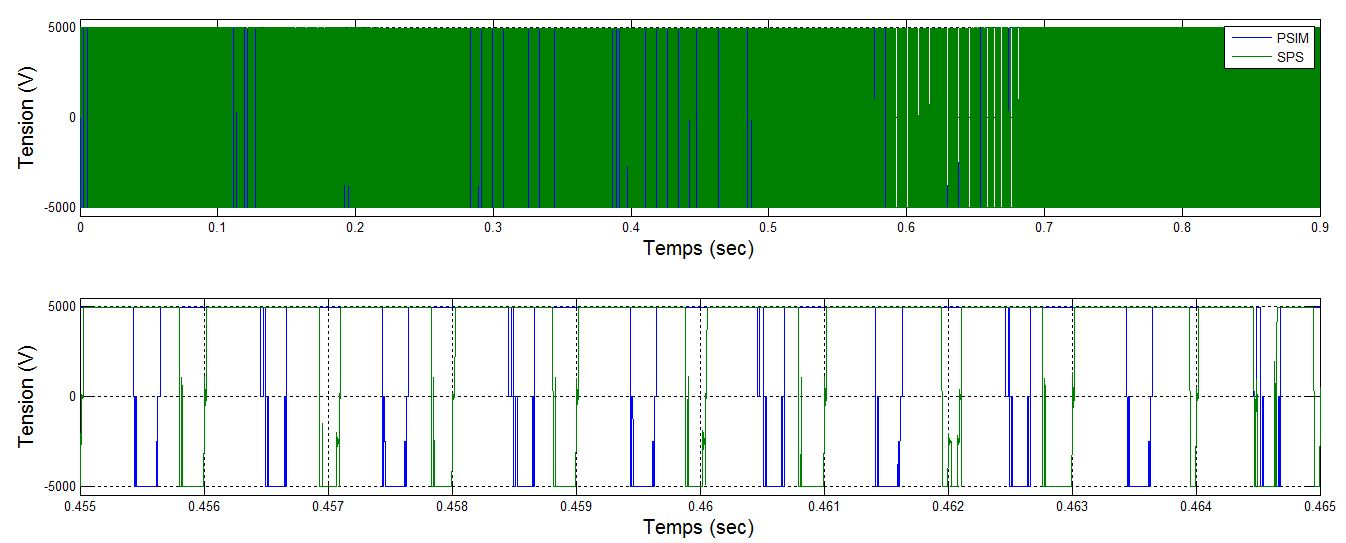
\includegraphics[scale=0.5]{Fig/DCPDCN/DCPTensionCharge1u.jpg}
\caption{Tension aux bornes de la charge sur PSIM et SPS pour un pas de calcul de 1$\mu$s}
\label{DC_ch_ten_1}
\end{figure}


\begin{figure}[htb]
\centering
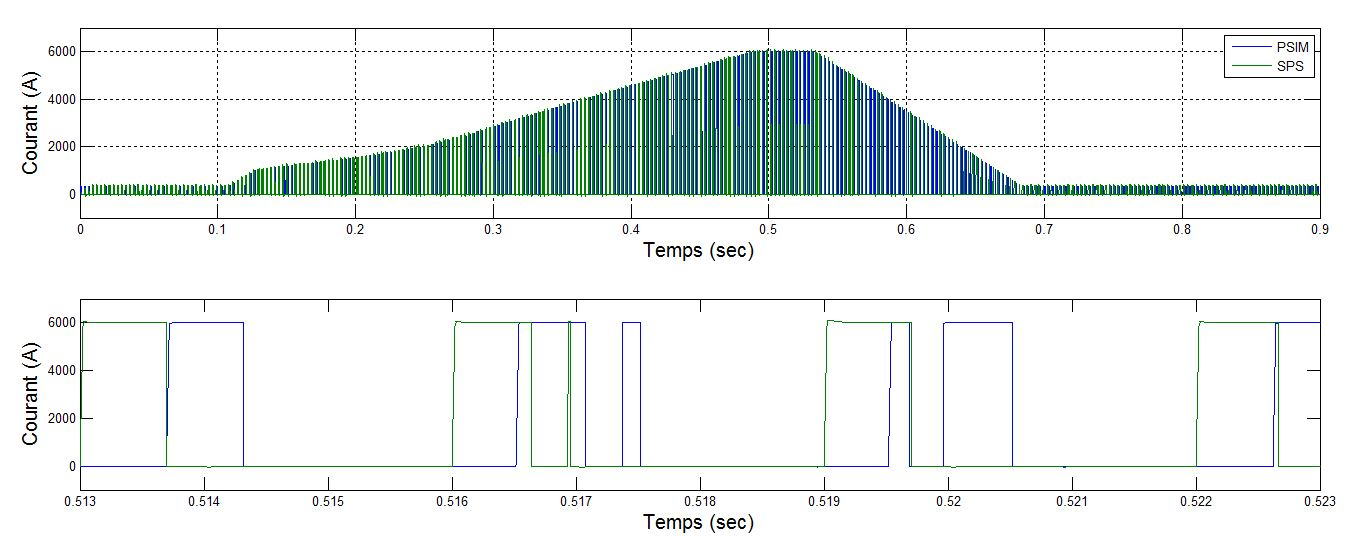
\includegraphics[scale=0.5]{Fig/DCPDCN/DCPCourantIGBT1u.jpg}
\caption{Courant traversant un IGBT sur PSIM et SPS pour un pas de calcul de 1$\mu$s}
\label{DC_IG_cou_1}
\end{figure}


\begin{figure}[htb]
\centering
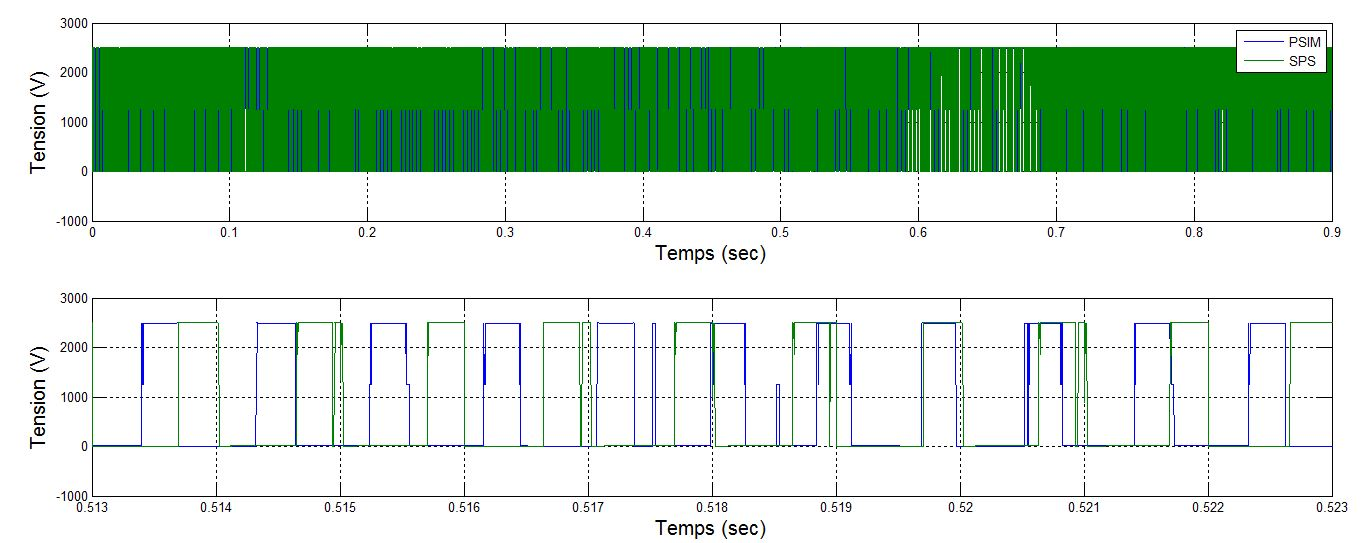
\includegraphics[scale=0.5]{Fig/DCPDCN/DCPTensionIGBT1u.jpg}
\caption{Tension aux bornes d'un IGBT sur PSIM et SPS pour un pas de calcul de 1$\mu$s}
\label{DC_IG_ten_1}
\end{figure}


\clearpage
\section{AFE: Validation PSIM/SPS}
\subsection{AFE source idéal}
L'AFE source idéal est constitué de 6 interrupteurs, soit deux par phase de tension. Ce système sert comme onduleur et sa tache est d'alimenter un bus CC pour qu'il ait une tension de 5000V. Ce sous-système sert à vérifier le fonctionnement 4 quadrant de l'AFE au niveau de l'échange de puissance. Il est composé d'une source AC d'un côté et DC parfaite de l'autre. Il est régulé en courant (Amplitude et phase) grâce à une régulation par hystérésis. La figure~\ref{AFE} est une représentation schématique de l'AFE source idéal. Il faut prendre en compte que ce sous-système ne contient pas les mêmes valeurs de paramètres pour le PI que la simulations de SPS, à cause que le calcul du RMS du courant sur PSIM n'est pas linéaire, le calcul de la moyenne de la valeur du RMS a été nécessaire. Tout ceci, fait en sorte que la dynamique du système n'était pas la même entre PSIM et SPS se qui a nécessite d'autres valeurs pour les PI.

\begin{figure}[htb]
\centering
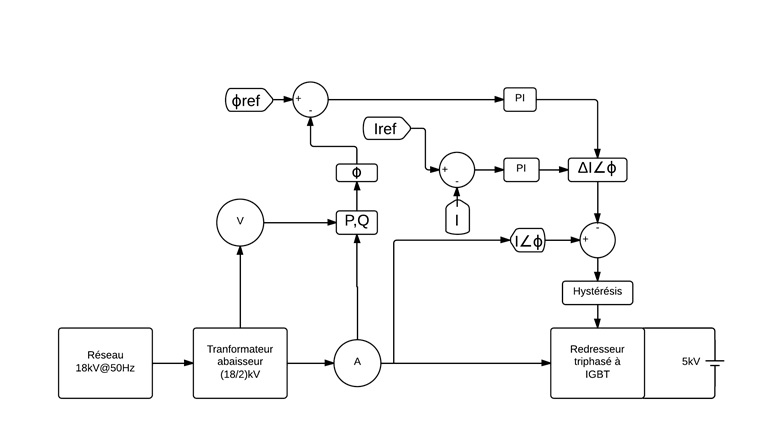
\includegraphics[scale=0.5]{Fig/AFEIDEAL/AFE.jpg}
\caption{Schéma bloc de l'AFE 2 level source parfaite avec régulation par hystérésis}
\label{AFE}
\end{figure}

\subsubsection{Vérification pour un pas de calcul de 1$\mu$s}
Cette section présente les courbes d'intérêt pour un pas de calcul discret de 1$\mu$s. La figure~\ref{AF_I_cou} représente le courant AC en entré de l'AFE pour un pas de calcul de 1$\mu$. On remarque que les courants sont très semblables entre eux. Mais sur PSIM, le courant a une région (proche de 0A)ou il contient moins d'oscillations comparés à celui de SPS.


\begin{figure}[htb]
\centering
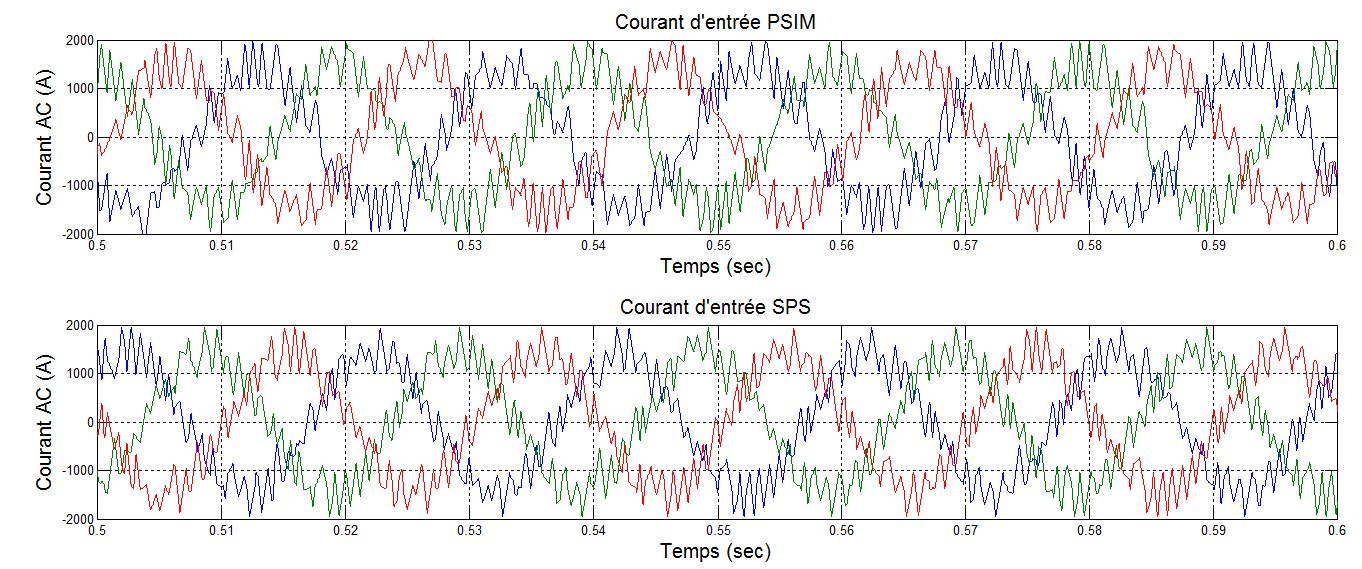
\includegraphics[scale=0.5]{Fig/AFEIDEAL/CourantAC.jpg}
\caption{Le courant d'entré à 1$\mu$s}
\label{AF_I_cou}
\end{figure}

Les figures~\ref{AF_I_pui_45}, ~\ref{AF_I_pui_135}, ~\ref{AF_I_pui__45} et ~\ref{AF_I_pui__135} représentent la puissance trouvé pour différentes phases de courant, ce qui montre que le système est capable fonctionner en 4 quadrants.

\begin{figure}[htb]
\centering
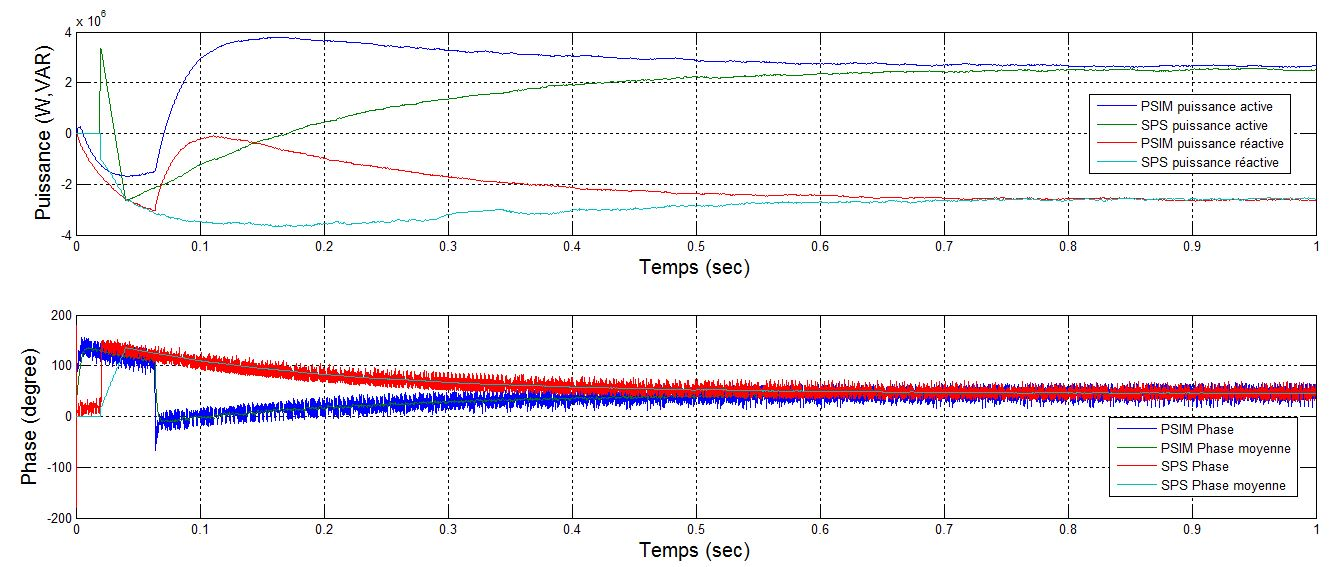
\includegraphics[scale=0.5]{Fig/AFEIDEAL/pui45.jpg}
\caption{La puissance à une phase de 45 degré à 1$\mu$s}
\label{AF_I_pui_45}
\end{figure}

\begin{figure}[htb]
\centering
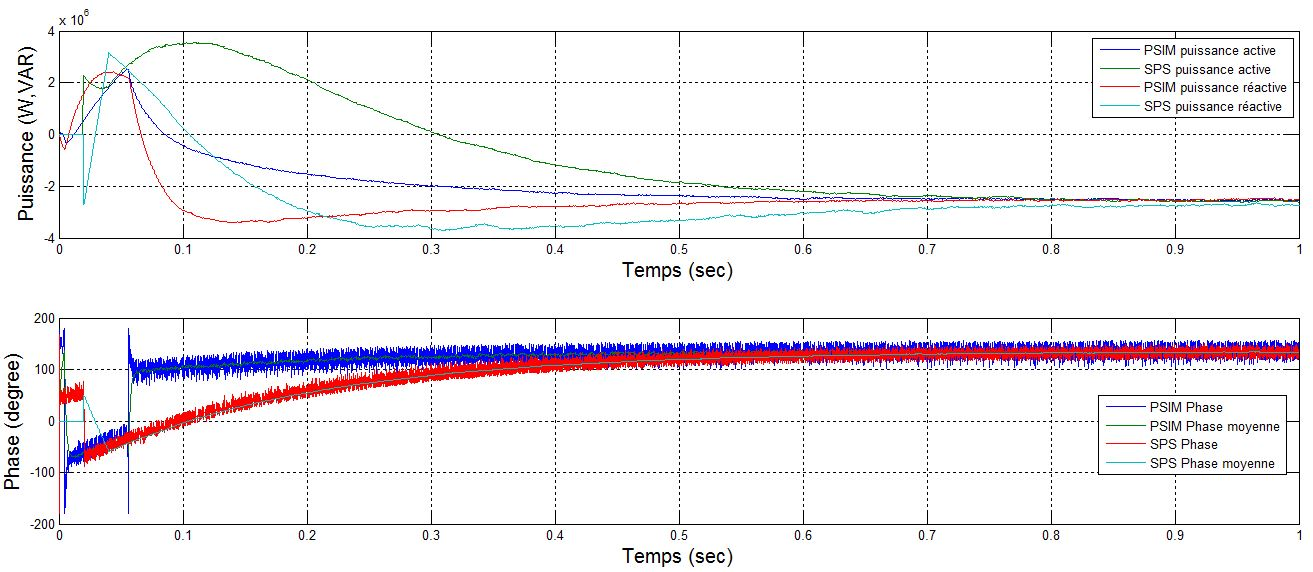
\includegraphics[scale=0.5]{Fig/AFEIDEAL/pui135.jpg}
\caption{La puissance à une phase de 135 degré à 1$\mu$s}
\label{AF_I_pui_135}
\end{figure}

\begin{figure}[htb]
\centering
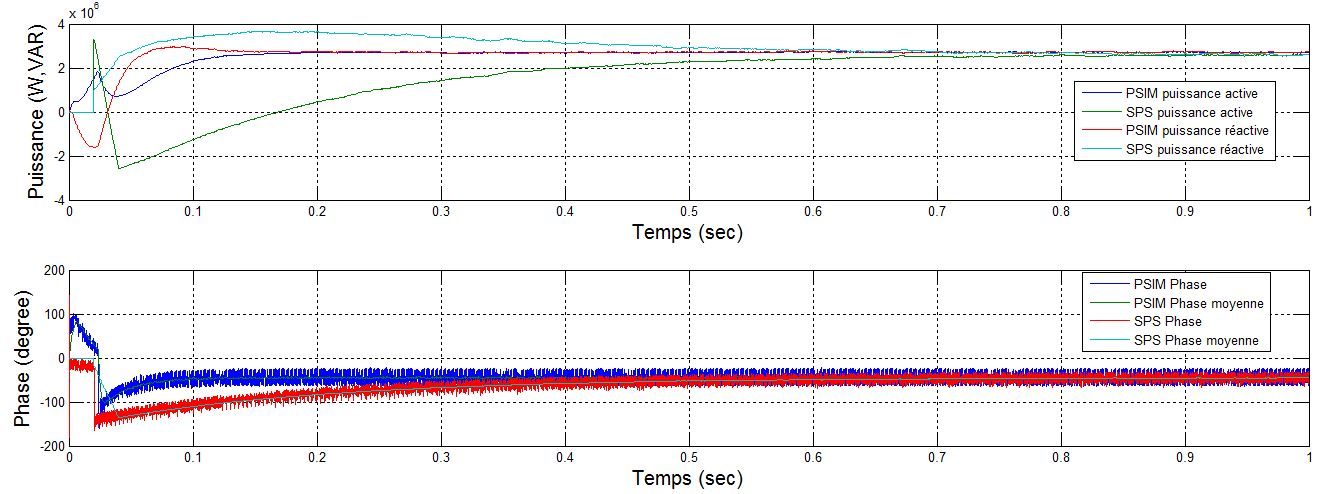
\includegraphics[scale=0.5]{Fig/AFEIDEAL/pui_45.jpg}
\caption{La puissance à une phase de -45 degré à 1$\mu$s}
\label{AF_I_pui__45}
\end{figure}

\begin{figure}[htb]
\centering
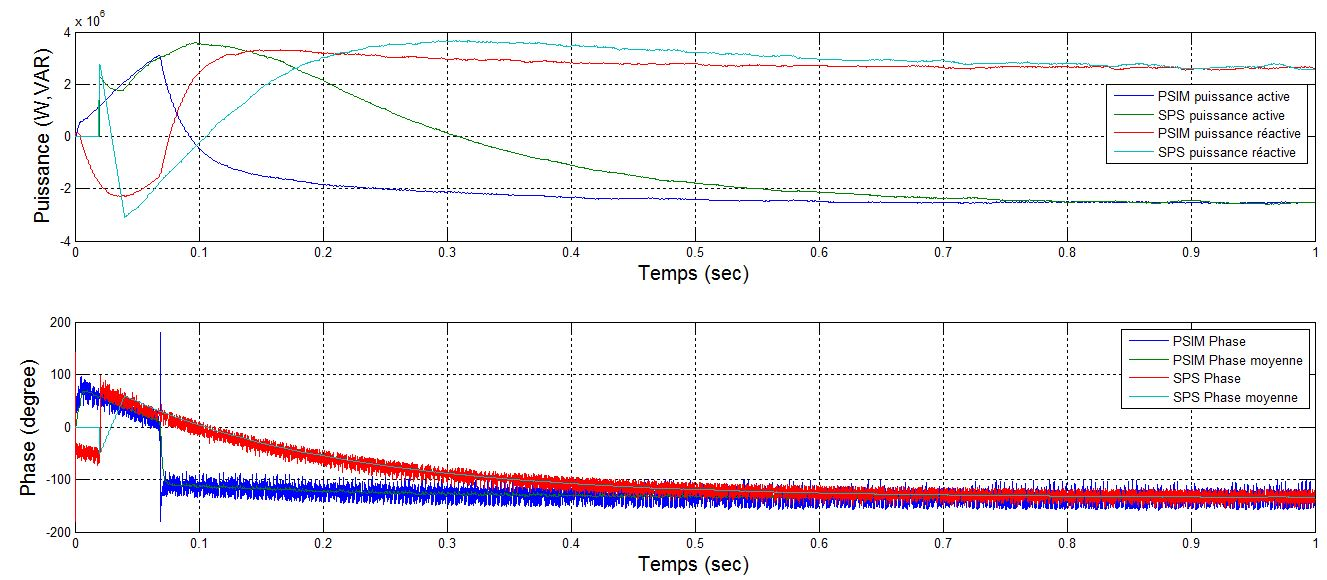
\includegraphics[scale=0.5]{Fig/AFEIDEAL/pui_135.jpg}
\caption{La puissance à une phase de -135 degré à 1$\mu$s}
\label{AF_I_pui__135}
\end{figure}


\clearpage
\subsection{AFE avec charge RC}
L'AFE avec charge RC est le même système que présenté dans la figure~\ref{AFE}. Les différences sont, qu'à la place d'une charge parfaite à 5000V, il est constitué d'une charge RC de 9.26$\Omega$ et 300mF.
De plus, le courant du réseau est mit en phase avec la tension du réseau. La figure~\ref{fft_RC} représente le calcul de fft d'une phase du courant d'entrée. Les paramètres de l'hystérésis ont été calibré pour que ça fréquence secondaire soit d'environs 1000Hz.

\begin{figure}[htb]
\centering
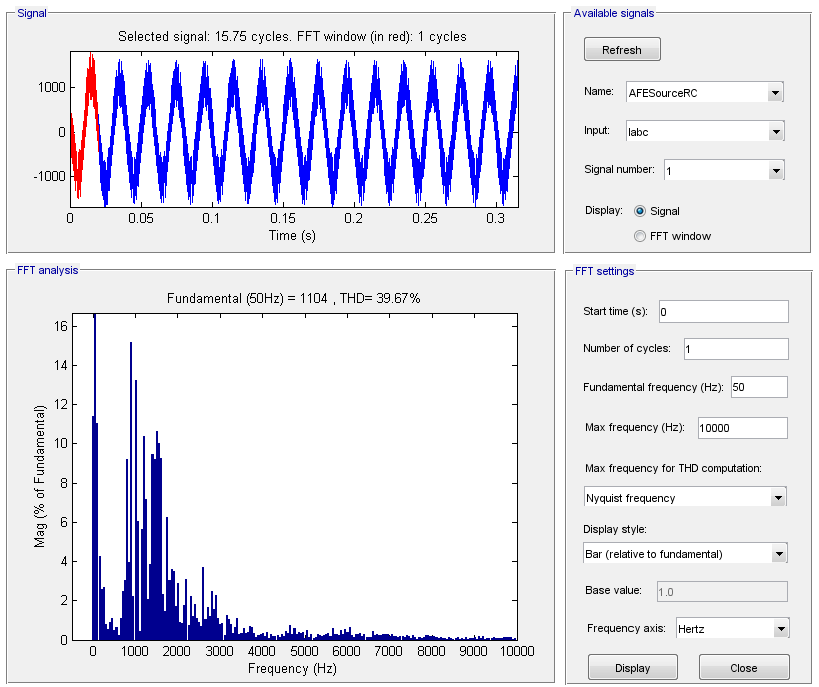
\includegraphics[scale=0.5]{Fig/AFERC/FFTAnalysisToolResult5u.png}
\caption{La FFT du courant d'entrée à 1$\mu$s}
\label{fft_RC}
\end{figure}


\subsubsection{Vérification pour un pas de calcul de 1$\mu$s}
Cette section présente les courbes d'intérêt pour un pas de calcul discret de 1$\mu$s. La figure~\ref{AF_RC_cou} représente le courant d'entré à un pas de calcul de 1$\mu$s. On observe une grosse différence au niveau du courant d'entré entre PSIM et SPS. SPS contient un courant d'entrée avec des oscillations régulières tandis que sur les simulations de PSIM le courant est irrégulier et ne comporte pas toujours des oscillations. Cette différence est causé à cause des 'Relay' utilisé sur PSIM qui ne sont pas modélisé de la même manière que ceux de SPS.




\begin{figure}[htb]
\centering
\includegraphics[scale=0.5]{Fig/AFERC/cour_al.jpg}
\caption{Le courant d'entré à 1$\mu$s}
\label{AF_RC_cou}
\end{figure}

La figure~\ref{AF_RC_ten} représente la tension au niveau de la charge. On observe une différence d'environs 7V entre le résultat de PSIM et celui de SPS. Cette différence est causé par des différences au sein de la dynamique des systèmes.


\begin{figure}[htb]
\centering
\includegraphics[scale=0.5]{Fig/AFERC/vch.jpg}
\caption{La tension à la charge à 1$\mu$s}
\label{AF_RC_ten}
\end{figure}

La figure~\ref{AF_RC_igbt} représente la tension et le courant aux bornes d'un IGBT. On observe que les résultats de tension sont assez semblables mais que pour le courant, il y a des moments ou le courant au niveau de PSIM n'atteint pas zéro et se remet à conduire. La différence vient entre autre de l'algorithme qui différe entre PSIM et SPS.

\begin{figure}[htb]
\centering
\includegraphics[scale=0.5]{Fig/AFERC/IGBT.jpg}
\caption{La tension et le courant au niveau d'un IGBT à 1$\mu$s}
\label{AF_RC_igbt}
\end{figure}


\clearpage
\subsection{AFE 3 niveau}
Ce système est composé de 12 interrupteurs IGBT ainsi que de 6 diodes de retour. Il est régulé grâce à une régulation par MLI.

\subsubsection{Vérification pour un pas de calcul de 50$\mu$s}
Cette section présente les courbes d'intérêt pour un pas de calcul discret de 50$\mu$s. La figure~\ref{AF_3_cou50} représente le courant d'entré de l'AFE 3 niveau avec un pas de calcul de 50$\mu$s. On remarque que le courant de SPS et PSIM sont pratiquement identique. 

\begin{figure}[htb]
\centering
\includegraphics[scale=0.5]{Fig/AFE3LEVEL/50u/cour_al.jpg}
\caption{Le courant d'entré à 50$\mu$s}
\label{AF_3_cou50}
\end{figure}

La figure~\ref{AF_3_vch50} représente la tension à la charge. Selon la figure, la tension de PSIM est d'environs 7V de moins que celle de SPS.
\begin{figure}[htb]
\centering
\includegraphics[scale=0.5]{Fig/AFE3LEVEL/50u/vch.jpg}
\caption{La tension à la charge à 50$\mu$s}
\label{AF_3_vch50}
\end{figure}

La figure~\ref{AF_3_IGBT50} représente la tension et le courant aux bornes d'un IGBT. Sur la figure, on remarque que le courant n'est pas à la même fréquence entre PSIM et SPS. La tension comporte des commutations non désiré.
\begin{figure}[htb]
\centering
\includegraphics[scale=0.5]{Fig/AFE3LEVEL/50u/IGBT.jpg}
\caption{La tension et le courant au niveau d'un IGBT à 50$\mu$s}
\label{AF_3_IGBT50}
\end{figure}

La figure~\ref{AF_3_DIODE50} représente la tension et le courant au bornes d'une diode. On remarque que sur PSIM la diode a des impulsions de courant négligeables ce que la courbe de SPS n'a pas. On remarque qu'il y présence de commutation non désirée.

\begin{figure}[htb]
\centering
\includegraphics[scale=0.5]{Fig/AFE3LEVEL/50u/DIODE.jpg}
\caption{La tension et le courant au niveau d'une diode à 50$\mu$s}
\label{AF_3_DIODE50}
\end{figure}

\clearpage
\subsubsection{Vérification pour un pas de calcul de 5$\mu$s}
Cette section présente les courbes d'intérêt pour un pas de calcul discret de 5$\mu$s. La figure~\ref{AF_3_cou5} représente le courant d'entré de l'AFE 3 niveaux à un pas de calcul de 5$\mu$s. Le courant observé est pratiquement identique entre PSIM et SPS.
\begin{figure}[htb]
\centering
\includegraphics[scale=0.5]{Fig/AFE3LEVEL/5u/cour_al.jpg}
\caption{Le courant d'entré à 5$\mu$s}
\label{AF_3_cou5}
\end{figure}
La figure~\ref{AF_3_vch5} représente la tension à la charge. Selon la figure, la tension de PSIM est d'environs 7V de moins que celle de SPS.
\begin{figure}[htb]
\centering
\includegraphics[scale=0.5]{Fig/AFE3LEVEL/5u/vch.jpg}
\caption{La tension à la charge à 5$\mu$s}
\label{AF_3_vch5}
\end{figure}
La figure~\ref{AF_3_IGBT5} représente la tension et le courant aux bornes d'un IGBT. Sur la figure, on remarque que le courant est décalé entre PSIM et SPS, il contient un décalage glissant. On remarque que la tension aux bornes de l'IGBT est très semblable. Il y présence d'un décalage temporelle glissant comme la courbe de courant.

\begin{figure}[htb]
\centering
\includegraphics[scale=0.5]{Fig/AFE3LEVEL/5u/IGBT.jpg}
\caption{La tension et le courant au niveau d'un IGBT à 5$\mu$s}
\label{AF_3_IGBT5}
\end{figure}

La figure~\ref{AF_3_DIODE5} représente la tension et le courant aux bornes de la diode de retour. On remarque que la tension a un décalage glissant entre PSIM et SPS. Le courant de PSIM comporte des impulsions tandis que SPS n'en contient pas.

\begin{figure}[htb]
\centering
\includegraphics[scale=0.5]{Fig/AFE3LEVEL/5u/DIODE.jpg}
\caption{La tension et le courant au niveau d'une diode à 5$\mu$s}
\label{AF_3_DIODE5}
\end{figure}

\clearpage
\subsubsection{Vérification pour un pas de calcul de 1$\mu$s}
Cette section présente les courbes d'intérêt pour un pas de calcul discret de 1$\mu$s. La figure~\ref{AF_3_cou} représente le courant d'entrée pour un AFE 3 niveaux à un pas de calcul de 1$\mu$s. On remarque que le courant entre PSIM et SPS sont très semblables.

\begin{figure}[htb]
\centering
\includegraphics[scale=0.5]{Fig/AFE3LEVEL/1u/cour_al.jpg}
\caption{Le courant d'entrée à 1$\mu$s}
\label{AF_3_cou}
\end{figure}
Sur la figure~\ref{AF_3_vch}, comme pour les autres pas de calculs, on remarque que la tension à charge de PSIM est d'environs 7V inférieure à celui de SPS.

\begin{figure}[htb]
\centering
\includegraphics[scale=0.5]{Fig/AFE3LEVEL/1u/vch.jpg}
\caption{La tension à la charge à 1$\mu$s}
\label{AF_3_vch}
\end{figure}
La figure~\ref{AF_3_IGBT} représente la tension et le courant aux bornes d'un IGBT. Les résultats sont très semblables, mais il y a présence de commutations non désirées. De plus, on remarque que le courant est décalé entre PSIM et SPS d'environs 100$\mu$s a son maximum, mais se phase entre eux quand le courant passe par zéro.

\begin{figure}[htb]
\centering
\includegraphics[scale=0.5]{Fig/AFE3LEVEL/1u/IGBT.jpg}
\caption{La tension et le courant au niveau d'un IGBT à 1$\mu$s}
\label{AF_3_IGBT}
\end{figure}
La figure~\ref{AF_3_DIODE} représente la tension et le courant aux bornes d'une diode de retour. On remarque que les résultats de PSIM a plus de commutations non désirée que celle de SPS. À ce pas de 1$\mu$s, on remarque que PSIM et SPS a des impulsions de courant.

\begin{figure}[htb]
\centering
\includegraphics[scale=0.5]{Fig/AFE3LEVEL/1u/DIODE.jpg}
\caption{La tension et le courant au niveau d'une diode à 1$\mu$s}
\label{AF_3_DIODE}
\end{figure}

\clearpage
\section{Implémentation AFE avec DCP/DCN}
\subsection{AFE 2 level avec hacheur 4 quadrants}
Cette section va discuter des différences entre les résultat de simulations pour l'implémentation finale entre l'AFE 2 niveaux et le hacheur 4 quadrants. La figure~\ref{AF_DC} représente l'implémentation des deux sous-systèmes d'une façon schématique.
\begin{figure}[htb]
\centering
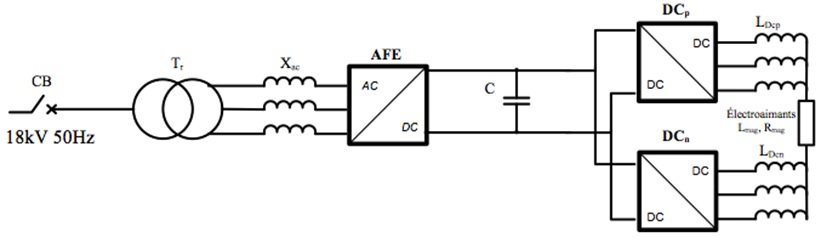
\includegraphics[scale=0.5]{Fig/Hach_AFE/AFE.jpg}
\caption{Représentation schématique de l'implémentation de l'AFE et du DCP/DCN}
\label{AF_DC}
\end{figure}


\subsubsection{Vérification pour un pas de calcul de 50$\mu$s}
Cette section présente les courbes d'intérêt pour un pas de calcul discret de 50$\mu$s. La figure~\ref{AF_HA_cou50} représente le courant d'entré au niveau de l'AFE 2 niveaux lorsqu'il est connecté au hacheur 4 quadrants. On remarque que le courant pour SPS est pointu tandis que celui de PSIm a des périodes ou le courant ne varie pas vraiment.

\begin{figure}[htb]
\centering
\includegraphics[scale=0.5]{Fig/Hach_AFE/50u/cour_al.jpg}
\caption{Le courant d'entré à 50$\mu$s}
\label{AF_HA_cou50}
\end{figure}

La figure~\ref{AF_HA_vch50} représente la tension au niveau du bus CC. On remarque que la tension du bus CC de SPS descend d'environs 100V plus bas que la tension de PSIM.
\begin{figure}[htb]
\centering
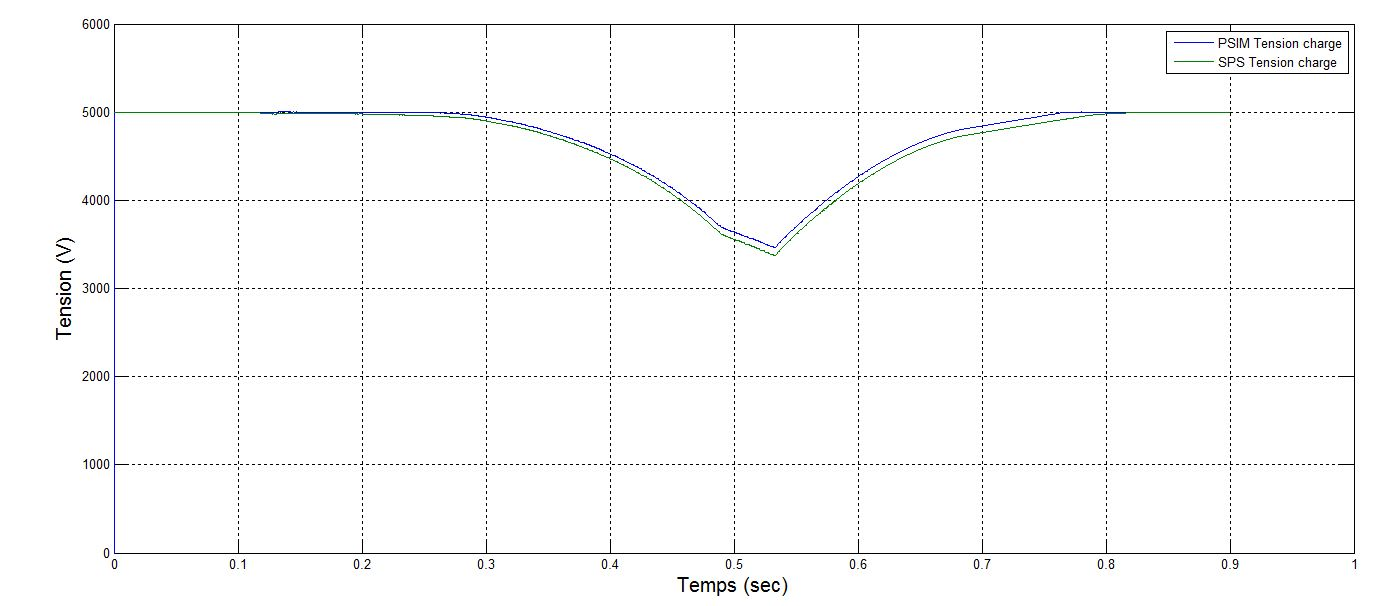
\includegraphics[scale=0.5]{Fig/Hach_AFE/50u/ten_bus.jpg}
\caption{La tension au bus à 50$\mu$s}
\label{AF_HA_vch50}
\end{figure}

La figure~\ref{AF_HA_IGBT50} représente la tension et le courant aux bornes d'un IGBT de l'AFE. On remarque une différence au niveau du courant qui est causé à cause de la différence de la forme de courant entre PSIM et SPS. 

\begin{figure}[htb]
\centering
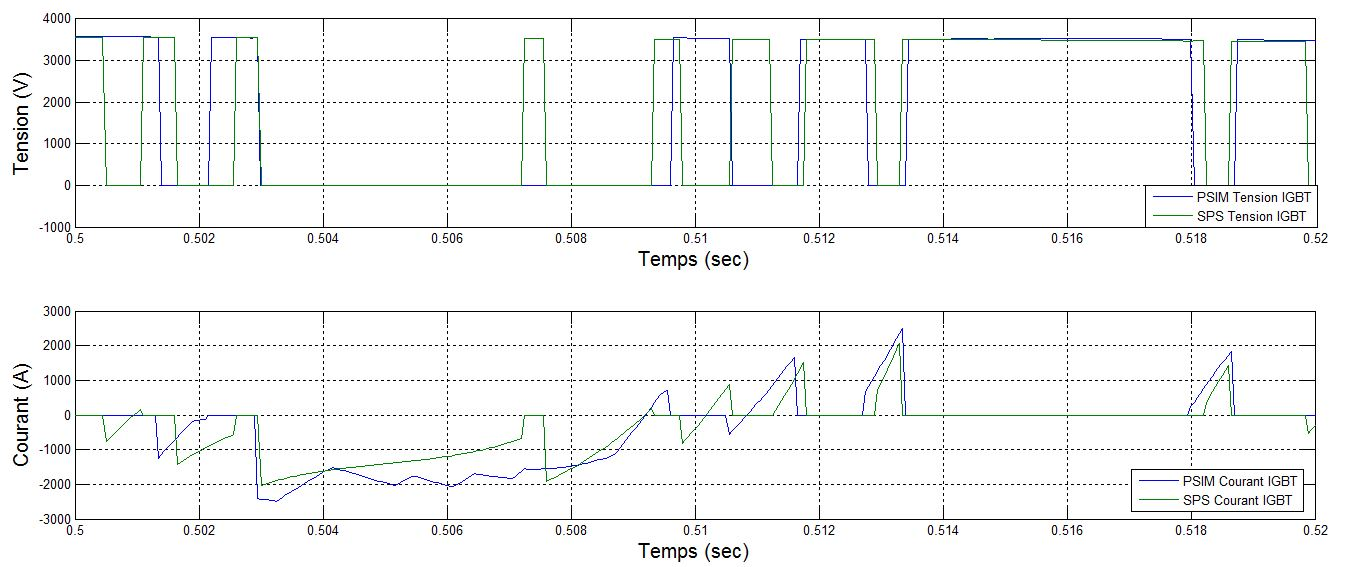
\includegraphics[scale=0.5]{Fig/Hach_AFE/50u/IGBT_AFE.jpg}
\caption{La tension et le courant au niveau d'un IGBT à 50$\mu$s au niveau de l'AFE}
\label{AF_HA_IGBT50}
\end{figure}
La figure~\ref{AF_HA_CHA50} représente le courant au niveau de la charge pour un pas de calcul de 50$\mu$. On remarque un décalage d'environs  100$\mu$s vers la droite du courant de SPS par rapport a celui de PSIM et de 50A entre eux. De plus, le courant est décalé d'environs 100A par rapport à la référence voulu. 

\begin{figure}[htb]
\centering
\includegraphics[scale=0.5]{Fig/Hach_AFE/50u/hach_cou_ch.jpg}
\caption{Le courant au niveau de la charge à 50$\mu$s}
\label{AF_HA_CHA50}
\end{figure}

La figure~\ref{AF_HA_CHV50} représente la tension aux bornes de la charge. On remarque que les résultats entre les deux simulations sont semblables à part le fait que la tension de SPS est décalé d'environs 100$\mu$s vers la droite. 

\begin{figure}[htb]
\centering
\includegraphics[scale=0.5]{Fig/Hach_AFE/50u/hach_ten_ch.jpg}
\caption{La tension au niveau de la charge à 50$\mu$s}
\label{AF_HA_CHV50}
\end{figure}

La figure~\ref{AF_HA_HAA50} représente le courant au bornes d'un IGBT. On remarque que les impulsions de courant sont très semblables,mais que la largeur des impulsions de courant ne sont pas de la même largeur et que la largeur des impulsions de courant de SPS et PSIM varient. Cette différence est causé par une différence au niveau de l'algorithme utilisé.

\begin{figure}[htb]
\centering
\includegraphics[scale=0.5]{Fig/Hach_AFE/50u/IGBT_cou_hach.jpg}
\caption{Le courant au niveau d'un IGBT à 50$\mu$s pour le hacheur 4 quadrants}
\label{AF_HA_HAA50}
\end{figure}

La figure~\ref{AF_HA_HAV50} représente la tension aux bornes d'un IGBT. On remarque que les résultats ont la même fréquence mais qui diffèrent en largeur.


\begin{figure}[htb]
\centering
\includegraphics[scale=0.5]{Fig/Hach_AFE/50u/IGBT_ten_hach.jpg}
\caption{La tension au niveau d'un IGBT à 50$\mu$s pour le hacheur 4 quadrants}
\label{AF_HA_HAV50}
\end{figure}

\clearpage
\subsubsection{Vérification pour un pas de calcul de 5$\mu$s}
Cette section présente les courbes d'intérêt pour un pas de calcul discret de 5$\mu$s. La figure~\ref{AF_HA_cou5} représente le courant d'entré pour un pas de calcul de 5$\mu$s. On remarque des différences entre les résultats de PSIM et SPS. Les résultats entre les courants de phase de SPS est pratiquement symétrique tandis que pour ceux de PSIM les oscillations sur le courant est aléatoire. Les deux ont pratiquement la même amplitude, mais les oscillations le courant sont très différentes.


\begin{figure}[htb]
\centering
\includegraphics[scale=0.5]{Fig/Hach_AFE/5u/cour_al.jpg}
\caption{Le courant d'entré à 5$\mu$s}
\label{AF_HA_cou5}
\end{figure}

La figure~\ref{AF_HA_vch5} représente la tension aux bornes du bus CC. On remarque que la tension sur SPS descend d'environs 50V plus bas que celle de PSIM.

\begin{figure}[htb]
\centering
\includegraphics[scale=0.5]{Fig/Hach_AFE/5u/ten_bus.jpg}
\caption{La tension au bus à 5$\mu$s}
\label{AF_HA_vch5}
\end{figure}

La figure~\ref{AF_HA_IGBT5} représente la tension et le courant aux bornes d'un IGBT au niveau de l'AFE. On remarque que les impulsions ne se déroule pas au même moment et le résultat de SPS a plus d'impulsions donc la forme de courant a des coupures pointus tandis que sur la courbe de courant de PSIM la forme est non linéaire.

\begin{figure}[htb]
\centering
\includegraphics[scale=0.5]{Fig/Hach_AFE/5u/IGBT_AFE.jpg}
\caption{La tension et le courant au niveau d'un IGBT à 5$\mu$s au niveau de l'AFE}
\label{AF_HA_IGBT5}
\end{figure}

La figure~\ref{AF_HA_CHA5} représente le courant au niveau de la charge. On remarque que le courant suit très bien la courbe de référence avec une oscillation d'environs 18A. De plus en remarque que le courant de PSIM est en phase avec celui de SPS. Les deux résultats de courant sont décalé d'environs 18A. 

\begin{figure}[htb]
\centering
\includegraphics[scale=0.5]{Fig/Hach_AFE/5u/hach_cou_ch.jpg}
\caption{Le courant au niveau de la charge à 5$\mu$s}
\label{AF_HA_CHA5}
\end{figure}

La figure~\ref{AF_HA_CHV5} représente la tension aux bornes de la charge. On remarque que les courbes de SPS et PSIM se superpose bien et sont pratiquement identique. La même chose se produit par rapport au courant et à la tension aux bornes de l'IGBT du hacheur 4 quadrants qui correspondent aux figures~\ref{AF_HA_HAA5} et ~\ref{AF_HA_HAV5}.

\begin{figure}[htb]
\centering
\includegraphics[scale=0.5]{Fig/Hach_AFE/5u/hach_ten_ch.jpg}
\caption{La tension au niveau de la charge à 5$\mu$s}
\label{AF_HA_CHV5}
\end{figure}



\begin{figure}[htb]
\centering
\includegraphics[scale=0.5]{Fig/Hach_AFE/5u/IGBT_cou_hach.jpg}
\caption{Le courant au niveau d'un IGBT à 5$\mu$s pour le hacheur 4 quadrants}
\label{AF_HA_HAA5}
\end{figure}

\begin{figure}[htb]
\centering
\includegraphics[scale=0.5]{Fig/Hach_AFE/5u/IGBT_ten_hach.jpg}
\caption{La tension au niveau d'un IGBT à 5$\mu$s pour le hacheur 4 quadrants}
\label{AF_HA_HAV5}
\end{figure}


\clearpage
\subsubsection{Vérification pour un pas de calcul de 1$\mu$s}
Cette section présente les courbes d'intérêt pour un pas de calcul discret de 1$\mu$s. La figure~\ref{AF_HA_cou1} représente le courant d'entré pour un pas de calcul de 1$\mu$s. On remarque que le courant de SPS a la même amplitude et non les mêmes oscillations que celui de PSIM.


\begin{figure}[htb]
\centering
\includegraphics[scale=0.5]{Fig/Hach_AFE/1u/cour_al.jpg}
\caption{Le courant d'entré à 1$\mu$s}
\label{AF_HA_cou1}
\end{figure}

La figure~\ref{AF_HA_vch1} représente la tension du bus CC. On remarque que la tension de SPS est d'environs 50V plus bas que celle de PSIM au point le plus bas.

\begin{figure}[htb]
\centering
\includegraphics[scale=0.5]{Fig/Hach_AFE/1u/ten_bus.jpg}
\caption{La tension au bus à 1$\mu$s}
\label{AF_HA_vch1}
\end{figure}

La figure~\ref{AF_HA_IGBT1} représente la tension et le courant au niveau de l'IGBT de l'AFE. On remarque que la tension et le courant entre PSIM et SPS ne sont pas synchronisés et les impulsions sont de largeur différentes.

\begin{figure}[htb]
\centering
\includegraphics[scale=0.5]{Fig/Hach_AFE/1u/IGBT_AFE.jpg}
\caption{La tension et le courant au niveau d'un IGBT à 1$\mu$s au niveau de l'AFE}
\label{AF_HA_IGBT1}
\end{figure}

La figure~\ref{AF_HA_CHA1} représente le courant au niveau de la charge. On remarque que le courant suit très bien la courbe de référence avec une oscillation d'environs 18A. De plus en remarque que le courant de PSIM est en phase avec celui de SPS. Les deux résultats de courant sont décalé d'environs 18A. 

\begin{figure}[htb]
\centering
\includegraphics[scale=0.5]{Fig/Hach_AFE/1u/hach_cou_ch.jpg}
\caption{Le courant au niveau de la charge à 1$\mu$s}
\label{AF_HA_CHA1}
\end{figure}


La figure~\ref{AF_HA_CHV1} représente la tension aux bornes de la charge. On remarque que les courbes de SPS et PSIM se superpose bien et sont pratiquement identique. La même chose se produit par rapport au courant et à la tension aux bornes de l'IGBT du hacheur 4 quadrants qui correspondent aux figures~\ref{AF_HA_HAA1} et ~\ref{AF_HA_HAV1}. Une différence est l'amplitude de la tension aux bornes de IGBT qui est un peu plus élevé sur PSIM et SPS d'environs 50V.

\begin{figure}[htb]
\centering
\includegraphics[scale=0.5]{Fig/Hach_AFE/1u/hach_ten_ch.jpg}
\caption{La tension au niveau de la charge à 1$\mu$s}
\label{AF_HA_CHV1}
\end{figure}

\begin{figure}[htb]
\centering
\includegraphics[scale=0.5]{Fig/Hach_AFE/1u/IGBT_cou_hach.jpg}
\caption{Le courant au niveau d'un IGBT à 1$\mu$s pour le hacheur 4 quadrants}
\label{AF_HA_HAA1}
\end{figure}

\begin{figure}[htb]
\centering
\includegraphics[scale=0.5]{Fig/Hach_AFE/1u/IGBT_ten_hach.jpg}
\caption{La tension au niveau d'un IGBT à 1$\mu$s pour le hacheur 4 quadrants}
\label{AF_HA_HAV1}
\end{figure}

\clearpage
\subsection{AFE 3 niveaux avec le DCP/DCN}
Cette section va discuter des différences au niveau des résultats de simulation par rapport au système regroupant l'AFE 3 niveaux avec le DCP/DCN. La figure~\ref{AF_DC} représente un schéma de l'implémentation des deux systèmes.

\subsubsection{Vérification pour un pas de calcul de 50$\mu$s}
Cette section présente les courbes d'intérêt pour un pas de calcul discret de 50$\mu$s. La figure~\ref{AF_DC_cou50} représente le courant d'entré pour l'AFE 3 niveaux à un pas de calcul de 50$\mu$s.
On remarque que l'amplitude du courant d'entré de SPS est supérieure d'environs 300A par rapport à celui de PSIM,mais les oscillations sont très semblables.

\begin{figure}[htb]
\centering
\includegraphics[scale=0.5]{Fig/DCP_AFE/50u/cour_al.jpg}
\caption{Le courant d'entré à 50$\mu$s}
\label{AF_DC_cou50}
\end{figure}

La figure~\ref{AF_DC_vch50} représente la tension aux bornes du bus CC. On remarque que la tension du bus pour PSIM est d'environs 100V inférieure à celle de SPS à leur point le plus bas.

\begin{figure}[htb]
\centering
\includegraphics[scale=0.5]{Fig/DCP_AFE/50u/ten_bus.jpg}
\caption{La tension au bus à 50$\mu$s}
\label{AF_DC_vch50}
\end{figure}

La figure~\ref{AF_DC_IGBT50} représente la tension eet le courant aux bornes d'un IGBT au niveau de l'AFE. On remarque que l'IGBT contient des commutations non désiré autant pour PSIM que SPS. Les résultats ont un décalage glissant entre PSIM et SPS. 

\begin{figure}[htb]
\centering
\includegraphics[scale=0.5]{Fig/DCP_AFE/50u/IGBT_afe.jpg}
\caption{La tension et le courant au niveau d'un IGBT à 50$\mu$s au niveau de l'AFE}
\label{AF_DC_IGBT50}
\end{figure}

La figure~\ref{AF_DC_DI50} représente la tension et le courant aux bornes d'une diode de retour pour l'AFE. On remarque qu'il y a des commutations non désiré. Il y a présence d'impulsions de courant pour PSIM mais SPS n'en a pas et les impulsions de tensions diffère entre PSIM et SPS.

\begin{figure}[htb]
\centering
\includegraphics[scale=0.5]{Fig/DCP_AFE/50u/ten_diode_afe.jpg}
\caption{La tension et le courant au niveau d'une diode à 50$\mu$s au niveau de l'AFE}
\label{AF_DC_DI50}
\end{figure}

La figure~\ref{AF_DC_CHA50} représente le courant au bornes de la charge. On remarque que la fréquence des oscillations de courants n'est pas la même sur PSIM et SPS. Mais le courant suit très bien le courant de référence et oscille d'environs 18A. Le courant de PSIM et SPS sont identique à part le fait que leur fréquence ne le sont pas.

\begin{figure}[htb]
\centering
\includegraphics[scale=0.5]{Fig/DCP_AFE/50u/cour_ch.jpg}
\caption{Le courant au niveau de la charge à 50$\mu$s}
\label{AF_DC_CHA50}
\end{figure}

la figure~\ref{AF_DC_CHV50} représente la tension aux bornes de la charge. Ont remarque la présence de commutation non désirées et une différence au niveau de la largeur des impulsions de tensions.

\begin{figure}[htb]
\centering
\includegraphics[scale=0.5]{Fig/DCP_AFE/50u/ten_ch.jpg}
\caption{La tension au niveau de la charge à 50$\mu$s}
\label{AF_DC_CHV50}
\end{figure}

La figure~\ref{AF_DC_HAA50} représente le courant aux bornes d'un IGBT pour le DCP/DCN. Il y a présence de dépassement et de commutation non désiré.

\begin{figure}[htb]
\centering
\includegraphics[scale=0.5]{Fig/DCP_AFE/50u/hash_cou_IGBT.jpg}
\caption{Le courant au niveau d'un IGBT à 50$\mu$s pour le DCP/DCN}
\label{AF_DC_HAA50}
\end{figure}

La figure~\ref{AF_DC_HAV50} représente la tension aux bornes d'un IGBT pour le DCP/DCN. Il y a présence de dépassement et de commutation non désiré qui représente le constat que la figure~\ref{AF_DC_HV50} qui représente la tension aux bornes d'une diode.

\begin{figure}[htb]
\centering
\includegraphics[scale=0.5]{Fig/DCP_AFE/50u/hash_ten_IGBT.jpg}
\caption{La tension au niveau d'un IGBT à 50$\mu$s pour le DCP/DCN}
\label{AF_DC_HAV50}
\end{figure}
La figure~\ref{AF_DC_HA50} représente le courant aux bornes d'une diode de retour. Il y a présence d'impulsions de courant pour SPS et non pour PSIM.

\begin{figure}[htb]
\centering
\includegraphics[scale=0.5]{Fig/DCP_AFE/50u/hash_diode_cou.jpg}
\caption{Le courant au niveau d'une diode à 50$\mu$s pour le DCP/DCN}
\label{AF_DC_HA50}
\end{figure}


\begin{figure}[htb]
\centering
\includegraphics[scale=0.5]{Fig/DCP_AFE/50u/hash_diode.jpg}
\caption{La tension au niveau d'une diode à 50$\mu$s pour le DCP/DCN}
\label{AF_DC_HV50}
\end{figure}

\clearpage
\subsubsection{Vérification pour un pas de calcul de 5$\mu$s}
Cette section présente les courbes d'intérêt pour un pas de calcul discret de 5$\mu$s. La figure~\ref{AF_DC_cou5} représente le courant d'entré à un pas de calcul de 5$\mu$s. On remarque que le courant d'entré est très semblable entre PSIM et SPS.
\begin{figure}[htb]
\centering
\includegraphics[scale=0.5]{Fig/DCP_AFE/5u/cour_al.jpg}
\caption{Le courant d'entré à 5$\mu$s}
\label{AF_DC_cou5}
\end{figure}

LA figure~\ref{AF_DC_vch5} représente la tension au niveau du bus CC. On remarque que la courbe de PSIM superpose parfaitement celle de SPS.

\begin{figure}[htb]
\centering
\includegraphics[scale=0.5]{Fig/DCP_AFE/5u/ten_bus.jpg}
\caption{La tension au bus à 5$\mu$s}
\label{AF_DC_vch5}
\end{figure}

La figure~\ref{AF_DC_IGBT5} représente la tension et le courant au bornes d'un IGBT. On remarque les mêmes impulsions mais à largeur différente et pas au même moment entre PSIM et SPS.

\begin{figure}[htb]
\centering
\includegraphics[scale=0.5]{Fig/DCP_AFE/5u/IGBT_afe.jpg}
\caption{La tension et le courant au niveau d'un IGBT à 5$\mu$s au niveau de l'AFE}
\label{AF_DC_IGBT5}
\end{figure}

La figure~\ref{AF_DC_DI5} représente la tension et le courant au niveau d'une diode de retour. On remarque la présence d'une petite impulsion de courant pour PSIm et d'une grosse impulsion pour SPS. Les impulsions de tensions sont décalé et ne se déroule pas au même intervalle.

\begin{figure}[htb]
\centering
\includegraphics[scale=0.5]{Fig/DCP_AFE/5u/ten_diode_afe.jpg}
\caption{La tension et le courant au niveau d'une diode à 5$\mu$s au niveau de l'AFE}
\label{AF_DC_DI5}
\end{figure}

La figure~\ref{AF_DC_CHA5} représente le courant aux bornes de la charge. On remarque que le courant suit très bien le courant de référence et oscille d'environs 10A. Le courant de PSIM et SPS sont identique à part le fait qu'il sont décalé d'environs 250$\mu$s.

\begin{figure}[htb]
\centering
\includegraphics[scale=0.5]{Fig/DCP_AFE/5u/cour_ch.jpg}
\caption{Le courant au niveau de la charge à 5$\mu$s}
\label{AF_DC_CHA5}
\end{figure}

La figure~\ref{AF_DC_CHV5} représente la tension aux bornes de la charge. On remarque la présence de commutation non désiré.

\begin{figure}[htb]
\centering
\includegraphics[scale=0.5]{Fig/DCP_AFE/5u/ten_ch.jpg}
\caption{La tension au niveau de la charge à 5$\mu$s}
\label{AF_DC_CHV5}
\end{figure}

La figure~\ref{AF_DC_HAA5} représente le courant aux bornes d'un IGBT au niveau de DCP/DCN. Le courant de SPS contient des dépassements et est décalé vers la gauche par rapport à celui de PSIM de 800$\mu$s.

\begin{figure}[htb]
\centering
\includegraphics[scale=0.5]{Fig/DCP_AFE/5u/hash_cou_IGBT.jpg}
\caption{Le courant au niveau d'un IGBT à 5$\mu$s pour le DCP/DCN}
\label{AF_DC_HAA5}
\end{figure}

La figure~\ref{AF_DC_HAV5} représente la tension aux bornes d'un IGBT au niveau du DCP/DCN. Les impulsions de tensions de SPS sont décalé vers la droite d'environs 200$\mu$s par rapport à PSIM.

\begin{figure}[htb]
\centering
\includegraphics[scale=0.5]{Fig/DCP_AFE/5u/hash_ten_IGBT.jpg}
\caption{La tension au niveau d'un IGBT à 5$\mu$s pour le DCP/DCN}
\label{AF_DC_HAV5}
\end{figure}

La figure~\ref{AF_DC_HA5} représente le courant aux bornes d'une diode de retour au niveau du DCP/DCN. On remarque la présence d'impulsions de courant pour SPS et non pour PSIM.

\begin{figure}[htb]
\centering
\includegraphics[scale=0.5]{Fig/DCP_AFE/5u/hash_diode_cou.jpg}
\caption{Le courant au niveau d'une diode à 5$\mu$s pour le DCP/DCN}
\label{AF_DC_HA5}
\end{figure}

La figure~\ref{AF_DC_HV5} représente la tension aux bornes d'une diode de retour au niveau du DCP/DCN. Les impulsions de tensions de SPS sont décalé vers la droite d'environs 200$\mu$s par rapport à PSIM.

\begin{figure}[htb]
\centering
\includegraphics[scale=0.5]{Fig/DCP_AFE/5u/hash_diode.jpg}
\caption{La tension au niveau d'une diode à 5$\mu$s pour le DCP/DCN}
\label{AF_DC_HV5}
\end{figure}


\clearpage
\subsubsection{Vérification pour un pas de calcul de 1$\mu$s}
Cette section présente les courbes d'intérêt pour un pas de calcul discret de 1$\mu$s. La figure~\ref{AF_DC_cou1} représente le courant d'entré de l'AFE pour un pas de calcul de 1$\mu$s. On remarque que le courant est visiblement identique entre PSIM et SPS.

\begin{figure}[htb]
\centering
\includegraphics[scale=0.5]{Fig/DCP_AFE/1u/cour_al.jpg}
\caption{Le courant d'entré à 1$\mu$s}
\label{AF_DC_cou1}
\end{figure}

La figure~\ref{AF_DC_vch1} représente la tension aux bornes du bus CC. On remarque que la tension surPSIM est identique à celle de SPS.

\begin{figure}[htb]
\centering
\includegraphics[scale=0.5]{Fig/DCP_AFE/1u/ten_bus.jpg}
\caption{La tension au bus à 1$\mu$s}
\label{AF_DC_vch1}
\end{figure}

La figure~\ref{AF_DC_IGBT1} représente la tension et le courant aux bornes d'un IGBT au niveau de l'AFE. On remarque que le résultat est sensiblement le même entre PSIM et SPS à part un petit décalage d'environs 50$\mu$s.

\begin{figure}[htb]
\centering
\includegraphics[scale=0.5]{Fig/DCP_AFE/1u/IGBT_afe.jpg}
\caption{La tension et le courant au niveau d'un IGBT à 1$\mu$s au niveau de l'AFE}
\label{AF_DC_IGBT1}
\end{figure}

La figure~\ref{AF_DC_DI1} représente la tension et le courant aux bornes d'une diode de retour. On remarque une tension pratiquement identique entre PSIM et SPS et des impulsions de courant autant sur PSIM que sur SPS.

\begin{figure}[htb]
\centering
\includegraphics[scale=0.5]{Fig/DCP_AFE/1u/ten_diode_afe.jpg}
\caption{La tension et le courant au niveau d'une diode à 1$\mu$s au niveau de l'AFE}
\label{AF_DC_DI1}
\end{figure}

La figure~\ref{AF_DC_CHA1} représente le courant au niveau de la charge. On remarque que le courant sur PSIM et SPS suit parfaitement la référence de courant et ont la même amplitude d'oscillation d'environs 10A. La fréquence des oscillations de SPS est un peu plus grande que celle de PSIM.

\begin{figure}[htb]
\centering
\includegraphics[scale=0.5]{Fig/DCP_AFE/1u/cour_ch.jpg}
\caption{Le courant au niveau de la charge à 1$\mu$s}
\label{AF_DC_CHA1}
\end{figure}

La figure~\ref{AF_DC_CHV1} représente la tension aux bornes de la charge. On remarque la présence de commutation non désirée.

\begin{figure}[htb]
\centering
\includegraphics[scale=0.5]{Fig/DCP_AFE/1u/ten_ch.jpg}
\caption{La tension au niveau de la charge à 1$\mu$s}
\label{AF_DC_CHV1}
\end{figure}

Les figures~\ref{AF_DC_HAA1} et ~\ref{AF_DC_HAV1} représentent le courant et la tension aux bornes d'un IGBT au niveau du DCP/DCN. On remarque la présence de commutation non désirée et un décalage de PSIM vers la droite de 500$\mu$s par rapport à SPS.

\begin{figure}[htb]
\centering
\includegraphics[scale=0.5]{Fig/DCP_AFE/1u/hash_cou_IGBT.jpg}
\caption{Le courant au niveau d'un IGBT à 1$\mu$s pour le DCP/DCN}
\label{AF_DC_HAA1}
\end{figure}



\begin{figure}[htb]
\centering
\includegraphics[scale=0.5]{Fig/DCP_AFE/1u/hash_ten_IGBT.jpg}
\caption{La tension au niveau d'un IGBT à 1$\mu$s pour le DCP/DCN}
\label{AF_DC_HAV1}
\end{figure}

La figure~\ref{AF_DC_HA1} représente le courant aux bornes d'une diode de retour au niveau du DCP/DCN. On remarque la présence d'impulsions de courant pour SPS tandis que PSIM n'en a pas.

\begin{figure}[htb]
\centering
\includegraphics[scale=0.5]{Fig/DCP_AFE/1u/hash_diode_cou.jpg}
\caption{Le courant au niveau d'une diode à 1$\mu$s pour le DCP/DCN}
\label{AF_DC_HA1}
\end{figure}

La figure~\ref{AF_DC_HV1} représente la tension aux bornes d'une diode de retour au niveau du DCP/DCN. On remarque la présence de commutation non désirée. De plus, le résultat de PSIM est décalé vers la droite d'environs 500$\mu$s.

\begin{figure}[htb]
\centering
\includegraphics[scale=0.5]{Fig/DCP_AFE/1u/hash_diode.jpg}
\caption{La tension au niveau d'une diode à 1$\mu$s pour le DCP/DCN}
\label{AF_DC_HV1}
\end{figure}


\end{document}